\chapter{Estado de la Cuestión}
\label{cap:estadoDeLaCuestion}
En el presente capítulo se desarrollará la perspectiva teórica de la investigación llevada a cabo, para recuperar y transcender el conocimiento acumulado sobre las soluciones de modelado de lenguaje aplicado a la generación de historias de vida. El objetivo de este capítulo es habilitar una comprensión crítica sobre las propuestas obtenidas con el fin de tomar las decisiones necesarias para la construcción del sistema. 

La estructura de este capítulo gira entorno a varios puntos clave. En la primera sección, se realizará una aproximación a unos de los temas de este trabajo: las historias de vida como terapia de reminiscencia de la enfermedad de Alzheimer. Para continuar, antes de examinar los avances técnicos de la generación de lenguaje, se introducirá este campo de estudio a través de una breve descripción y un análisis de la evolución de las alternativas históricas para la generación de texto; continuando con la revisión de diferentes arquitecturas de sistemas de este tipo, en líneas generales. 

En las siguientes secciones, insistiremos en las técnicas más relevantes actualmente del panorama en el modelado de lenguaje, como método automático alternativo para la composición de historias de vida. 
Para ello, navegaremos a través de diferentes algoritmos neuronales ampliamente reconocidos en la composición de textos, desde los más avanzados y novedosos como los \textit{Transformers}, hasta construcciones más innovadoras en su aplicación a este campo.

\section{Alzheimer e historias de vida}
La pirámide poblacional modifica su estructura continuamente debido al progresivo envejecimiento generalizado de la población. En el año 2050, según proyecciones de la \cite{alzheimers-association-media-line-2021}, las personas mayores de 65 años constituirán el 16 por ciento de la población mundial frente al 8 por ciento del año 2010. El aumento de la esperanza de vida en todo el mundo, principalmente en las sociedades más avanzadas, y la disminución de la natalidad, se encuentran entre las causas de la modificación de la distribución demográfica hacia edades más avanzadas. Este fenómeno es conocido como \textit{inversión de la pirámide poblacional} \citep{RCSP892}.

La realidad detrás de estas estadísticas: el incremento del número de personas de edad avanzada; y asociándose al envejecimiento, la acumulación a lo largo del tiempo de una gran variedad de daños moleculares y celulares que llevan a un descenso gradual de las capacidades mentales y físicas, deriva en un mayor riesgo de determinadas enfermedades. 

La pérdida de la audición, las cataratas, la artritis y la artrosis son solo algunas de las enfermedades con mayor incidencia. Sin embargo, una de las dolencias más comunes dentro de este rango de población es la enfermedad de Alzheimer, cuya prevalencia a nivel global se espera que supere todo dato conocido hasta ahora, dado que se estima que en el año 2050 se incremente el número de casos a 152,8 millones, sobrepasando considerablemente los 57,4 millones del año 2019 \citep{alzheimers_disease_international_2019}.


\subsection{Descripción general}
La enfermedad de Alzheimer es un trastorno neurológico caracterizado por cambios degenerativos en diferentes sistemas neurotransmisores que abocan finalmente a la muerte de las células nerviosas del cerebro encargadas del almacenamiento y procesamiento de la información. Las regiones del cerebro involucradas con la memoria y los procesos de aprendizaje, asociadas a los lóbulos temporal y frontal, reducen su tamaño como consecuencia de la degeneración de las sinapsis y la muerte de las neuronas \citep{romano2007enfermedad,mattson2004pathways}. En las etapas finales de esta patología, este proceso, también denominado \textit{atrofia cerebral} se extiende y provoca una pérdida significativa del volumen cerebral (figura \ref{fig:CerebroPersonaAlzheimer} a).


\begin{figure}[!h]
	\centering%
	\includegraphics[width=0.8\textwidth]%
	{Imagenes/Vectorial/02EstadoDeLaCuestion/CerebroPersonaAlzheimer}%
	\caption{Reducción del cerebro asociada al Alzheimer \citep{mattson2004pathways}%
		\label{fig:CerebroPersonaAlzheimer}}
\end{figure}

En numerosas ocasiones son utilizadas imágenes similares a las mostradas en la figura \ref{fig:CerebroPersonaAlzheimer} como indicativos de la enfermedad del Alzheimer. La figura \ref{fig:CerebroPersonaAlzheimer} b  representa unas \textit{tomografías por emisión de positrones} o \textit{PET scans} en inglés. En ellas se reflejan los patrones de distribución espacial de la glucosa en el cerebro. En el cerebro de la persona con Alzheimer, el flujo glucolítico cerebral se minimiza provocando los síntomas de la enfermedad. Esta prueba se utiliza en el diagnóstico de la gravedad de la patología.


El proceso de detección de la enfermedad de Alzheimer es una tarea ardua de realizar dado que, por lo general, los síntomas iniciales de la enfermedad suelen atribuirse a un olvido puntual o la vejez, nada más lejos de la realidad. Según avanza la enfermedad, sus síntomas lo hacen con ella, agravándose y aumentando cada vez más hasta que el deterioro cognitivo ocasionado llega a afectar significativamente a las actividades de la vida diaria y finalmente a las necesidades fisiológicas básicas.

La evolución del Alzheimer se puede dividir en tres fases o etapas. En una primera instancia, se comienza a observar un deterioro cognitivo leve como puede ser la pérdida paulatina de la memoria episódica. Esta fase viene seguida de pérdidas de la memoria reciente, asociadas a un deterioro mayor, así como otras degeneraciones de funciones mentales y de la personalidad. Para terminar, se produce una pérdida progresiva de la memoria referida a los acontecimientos más antiguos, acompañando además un importante deterioro físico.


\subsection{Sintomatología y pérdida de la memoria}
La amnesia o pérdida de la memoria es uno de los síntomas más representativos del Alzheimer. Sin embargo, se trata tan solo de la punta del iceberg, debido a todos los desordenes que también se producen y que no son considerados o tenidos en cuenta por el personal no profesional: alteraciones del estado de ánimo y la conducta, dificultad de toma de decisiones, desorientación, problemas del lenguaje, dificultad para comer, movilidad reducida, y un largo etcétera son algunos de los síntomas que acompañan a esta enfermedad durante todo su camino. Todos estos síntomas dependen de la fase evolutiva de la enfermedad.

Podemos distinguir en cuanto a sintomatología dos fases marcadas por las alteraciones neurológicas: en la primera fase, conocida como fase predemencial, los signos de desordenes neurológicos todavía no se encuentran presentes; mientras que en la última fase, fase demencial, se pueden observar grandes alteraciones motoras, cognitivas, sensoriales y emocionales.

En la etapa predemencial, durante la cual el paciente puede no encontrarse aún diagnosticado de la enfermedad, comienzan a producirse lesiones microscópicas en el cerebro. Sin embargo, no es hasta entre 10 y 20 años después que pueden aparecer las primeras alteraciones cognitivas. El conjunto de síntomas presentes en esta fase comprende principalmente alteraciones en la conducta, tales como trastorno de la personalidad, apatía o cambios en el estado de ánimo; y deterioro gradual de la memoria, comenzando el paciente a olvidar pequeñas cosas y llegando a no ser capaz de recordar familia o amigos.

A medida que progresa el daño cerebral, aparece progresivamente un deterioro más pronunciado del paciente, comenzando entonces la fase demencial de la enfermedad. En esta etapa comienzan a aparecer alteraciones neurológicas como pérdida del movimiento, temblores, alucinaciones, trastornos en el lenguaje oral y escrito o alteraciones de la personalidad \citep{alberca-serrano-2010}.


\subsection{Tratamientos: historias de vida}
En la actualidad el Alzheimer es una enfermedad irreversible. Sin embargo, existen diversos tratamientos disponibles para ralentizar el avance de la enfermedad, así como mejorar la calidad de vida de los pacientes respecto a los síntomas. Estos tratamientos se pueden dividir en dos ramas diferenciadas: tratamientos farmacológicos o farmacoterapia, que se valen de medicamentos, y tratamientos no farmacológicos o psicosociales, que no hacen uso de sustancias químicas. Ambos tipos de tratamientos resultan eficaces para tratar la enfermedad de Alzheimer. Sin embargo, de la combinación de ambos resulta el procedimiento más recomendado debido a su mayor efectividad. Esto es posible gracias a que ambos tipos de tratamientos no son mutuamente excluyentes \citep{romano2007enfermedad}.

Existe una gran variedad de terapias no farmacológicas. Algunas de las más utilizadas son el entrenamiento y la estimulación cognitiva, el ejercicio físico o la musicoterapia. Además, dentro de cada una de estas terapias podemos encontrar una enorme cantidad de técnicas, siendo la reminiscencia la más utilizada como técnica de estimulación cognitiva.

Según \cite{o2013cross}, la reminiscencia es el acto o proceso de recordar sucesos, eventos o información del pasado. Esto puede implicar el recuerdo de episodios particulares o genéricos que pueden o no haber sido olvidados previamente, y que son acompañados por la sensación de que estos episodios son relatos verídicos de las experiencias originales. Esta técnica es empleada en la estimulación del la memoria episódica autobiográfica mediante el encadenamiento de recuerdos, que se agrupan en categorías y se archivan en el tiempo mediante la elaboración de la \textit{historia de vida}.

La historia de vida es una técnica narrativa que se basa en organizar y estructurar recuerdos de una persona para componer una autobiografía. Según \cite{linde1993life}, una historia de vida debe cumplir dos criterios: primero, debe incluir algunos puntos de evaluación que comuniquen los valores morales de la persona; y segundo, los eventos incluidos en la historia de vida deben tener un significado especial y ser de importancia para ella. Estos eventos deben ser aspectos significativos de la vida pasada de la persona, su presente y su futuro.

Para componer la historia de vida de una persona con Alzheimer se recopilan historias a través de familiares u otras personas cercanas. Posteriormente, se documentan en forma de un libro o cuaderno, incluyendo experiencias y logros junto con fotografías y escritos sobre hechos importantes para la vida de la persona, a través de los cuales se muestra quién es esa persona.

Cada persona tiene su propia historia de vida única. Nuestras experiencias nos modelan y construyen la persona que somos. Las historias de vida ayudan a las personas con Alzheimer a conectar con su identidad recordando épocas felices. El miedo y la frustración provocados por el olvido de las tareas de la vida cotidiana, nombres y rostros, se mitigan recordando quiénes eran a través de estas historias. Les ayuda a ser conscientes de los momentos especiales que han marcado su vida, las personas que han conocido en su infancia o trabajo. También pueden ser utilizados por los cuidadores para comprender más sobre ellos, quiénes son, y ayudarles en la reminiscencia de recuerdos \citep{karlsson2014stories}.


Existen diferentes formatos en los que se pueden registrar estas experiencias de la persona. Ninguno de ellos es mejor o peor que otro, sino que lo ideal es utilizar aquel que mejor se adapte a la persona y a los hechos que se quieran transmitir.

Por una parte encontramos historias de vida más visuales, compuestas enteramente de imágenes (\textit{collages}) o videos, dirigidas especialmente a las personas con Alzheimer que se encuentran en una etapa tardía de la enfermedad. Otro formato se centra especialmente en textos. Los \textit{libros de vida}, destinados a los cuidadores y visitantes tanto como a la propia persona, combina las \textit{historias de vida}, en forma de texto claro y fácil de leer, con algunas imágenes. También nos encontramos los documentos de perfil personal que se centran en pequeñas versiones cortas de las historias de vida excluyendo las imágenes. Estos documentos son utilizados a menudo en hospitales y están diseñados para ayudar al personal a comprender las necesidades de la persona.

El contenido de una historia de vida es variable, aunque existen algunos temas básicos en los que se debe centrar: el perfil de la persona, incluyendo datos e información básica como es el nombre, edad, lugar de nacimiento o de residencia son esenciales para aproximarse de manera inicial a la persona. Otros temas como las relaciones significativas familiares y de amistad, infancia, lugares y eventos significativos y gustos o preferencias y aficiones son incluidos dentro de esta lista de posibles temas a tratar el la historia de vida \citep{thompsonlifestory}.

\section{Generación de lenguaje natural}

La Generación de Lenguaje Natural (GLN) es un campo del Procesamiento de Lenguaje Natural (PLN) se define como el ``subcampo de la inteligencia artificial y la lingüística computacional que se ocupa de la construcción de sistemas informáticos que pueden producir textos comprensibles en inglés u otros lenguajes humanos a partir de alguna representación no lingüística subyacente de la información''  \citep{reiter1997building}. Si bien esta definición estuvo generalmente aceptada como la más conveniente al hablar de generación de lenguaje natural durante muchos años, \cite{gatt2018survey} puntualizan que es una afirmación que solo engloba una parte de la generación de textos, ya que se refiere únicamente a aquellos sistemas cuya entrada es una ``representación no lingüística [...] de la información'' o datos, como veremos más adelante en el apartado \ref{cap:nglD2T}.

Desde hace muchos años, la GLN es empleada en numerosos proyectos de distinta naturaleza como la traducción de textos \citep{Cho2014LearningPR}, realización de resúmenes y fusión de documentos \citep{clarke2010discourse}, corrección automática de ortografía y gramática \citep{islam2018bangla}, redacción de noticias \citep{leppanen2017data}, informes meteorológicos \citep{sripada2014case} y financieros \citep{ren2021hybrid}, generación de resúmenes sobre la información de recién nacidos en un contexto clínico \citep{BabyTalk}... Todos estos sistemas tienen en común la generación de un texto (normalmente de una alta calidad) a partir de muy diferentes fuentes de información.

\subsection{Clasificación de sistemas según el formato de entrada}
En los ejemplos de proyectos listados con anterioridad que emplean la generación de lenguaje natural para redactar diferentes tipos de texto, los datos utilizados como fuente de información son muy dispares, no solo en su contenido sino también en la forma. Así, para la traducción automática se emplea una entrada escrita en lenguaje natural, mientras que en otros sistemas como la creación de informes meteorológicos, se emplea información no lingüística. De esta manera, en lo que al tipo de entrada se refiere, se consideran dos enfoques diferenciados en los sistemas de generación de lenguaje: enfoques texto a texto (\textit{text-to-text}) y enfoques dato a texto (\textit{data-to-text}).

\subsubsection{Generación \textit{text-to-text} (T2T)}
Los sistemas de generación texto a texto, conocidos como \textit{text-to-text} en inglés o T2T por sus siglas, toman textos escritos en lenguaje natural como entrada y producen un texto nuevo y coherente como salida. La entrada de estos sistemas puede abarcar desde pequeñas oraciones a extensos escritos. Existen muchas aplicaciones en los sistemas GLN que utilizan T2T. Además de los mencionados anteriormente, pertenecen a este tipo la fusión de documentos y generación de resúmenes \citep{clarke2010discourse}, simplificación de textos complejos \citep{sulem2018simple}, o autocorrectores gramaticales \citep{Ge2019AutomaticGE}, entre otros. 

Sin embargo, el ejemplo más claro de este tipo de generación de lenguaje corresponde a un traductor automático. Este tipo de sistema ampliamente utilizado en la vida cotidiana toma una entrada textual correspondiente a un escrito en un idioma y genera un texto de salida en otro idioma. La traducción automática es un proceso muy complejo, puesto que no solamente tiene en cuenta el significado del corpus, sino que también hace falta interpretar y analizar de manera correcta todos los elementos del texto, así como comprender la influencia de unas palabras en otras con la finalidad de  generar un texto fluido y coherente.

\begin{figure}[!h]
	\centering
	%
	\begin{SubFloat}
		{\label{fig:inputFoG}%
			Entrada del sistema FoG}%
		\includegraphics[width=0.7\textwidth]%
		{Imagenes/Bitmap/02EstadoDeLaCuestion/inputFoG}%
	\end{SubFloat}
	\qquad
	\begin{SubFloat}
		{\label{fig:outputFoG}%
			Salida del sistema FoG}%
		\includegraphics[width=0.7\textwidth]%
		{Imagenes/Bitmap/02EstadoDeLaCuestion/outputFoG}%
	\end{SubFloat}
	\caption{Sistema \textit{data-to-text} FoG%
		\label{fig:FoG}}
\end{figure}

\subsubsection{Generación \textit{data-to-text} (D2T)}\label{cap:nglD2T}
Estos tipos de sistemas permiten la generación de texto como salida a partir de entradas no puramente textuales. Además, el formato de los datos que pueden tomar como entrada son muy diversos. Aunque es muy común encontrar sistemas que parten de datos numéricos como hojas de cálculo, hay que considerar otros orígenes de datos de tipo estructurado tales como bases de datos, simulaciones de sistemas físicos o grafos de conocimientos. De manera general, podemos referirnos a la representación de la información de esta clase de sistema como datos estructurados o procesables.


Uno de los ejemplos tradicionales más visuales que nos permite comprender este tipo de sistema, sería el \textit{Forecast Generator}, sistema que forma parte del \textit{Forecaster's Production Assistant}, entorno desarrollado por \textit{CoGenTex} en 1992 para \textit{Environment Canada} con el fin ayudar a los meteorólogos a aumentar su productividad al redactar por ellos un informe meteorológico textual en inglés y en francés \citep{goldberg1994using}. En la figura  \ref{fig:inputFoG} se muestra el entorno sobre el que los meteorólogos modifican valores como la presión atmosférica, situación de frentes y otros datos (datos no textuales). Una vez se pulsa sobre \textit{Generar}, el sistema muestra el texto correspondiente al informe (figura \ref{fig:outputFoG}). 


En la figura \ref{fig:data-to-text}, explicada con más detalle en \cite{sai2020survey}, se muestran los datos de entrada y de salida de un sistema GLN D2T acercándonos a la generación de lenguaje desde una perspectiva distinta al ejemplo explicado anteriormente. Los datos de entrada de este tipo de sistema toman la forma de grafo o cualquier otro tipo de datos semiestructurados como tablas (conjunto de tuplas del tipo [entidad, atributo, valor]). En la fila inferior, se muestran diferentes posibles soluciones como salida del sistema. En su trabajo, el autor introduce además la necesidad de métodos de evaluación de la calidad del texto redactado ya que de las diferentes salidas, solo la tercera opción cubre toda la información de entrada y resulta ser fluida.


\begin{figure}[!h]
	\centering%
	\includegraphics[width=1.0\textwidth]%
	{Imagenes/Bitmap/02EstadoDeLaCuestion/data-to-text}%
	\caption{Ejemplo de D2T utilizado por \cite{sai2020survey}%
		\label{fig:data-to-text}}
\end{figure}

\subsection{Historia de la generación de lenguaje}
Antes de adentrarnos en profundidad en otros conceptos de la generación de lenguaje, es conveniente conocer la evolución histórica del campo del Procesamiento de Lenguaje Natural dentro del que se engloba la generación de lenguaje, a modo de aproximación que nos permita el conocimiento del contexto de ciertas técnicas que se considerarán más adelante. En general, la historia del procesamiento de lenguaje natural, y por tanto de la generación de lenguaje, se divide en dos grandes períodos marcados por la aparición del aprendizaje profundo o \textit{Deep Learning} \citep{louis-2021}. 

La era \textit{pre Deep Learning} (figura \ref{fig:erapreDL}) comienza aproximadamente en el 1949, momento en el que Warren Weaver sugería en su memorando \textit{Translation} \footnote{Lectura disponible en https://aclanthology.org/www.mt-archive.info/90/MTNI-1999-Hutchins.pdf} que la traducción automática computacional era posible. Este trabajo constituyó la primera aproximación estadística al procesamiento y generación de lenguaje. Además, supuso una revolución e inspiró numerosos experimentos y proyectos que probaron que realmente esto era posible aunque a muy pequeña escala. Estos sistemas se basaban principalmente en la búsqueda en diccionarios de las palabras necesarias para la traducción y la posterior reordenación de las palabras para ajustarse a las reglas sintácticas del idioma destino de la traducción.

Después de una década de investigaciones para conseguir mejores resultados en este campo y de pérdida de financiación, ya que las soluciones encontradas conseguían resultados paupérrimos y decididamente insatisfactorios, surgieron avances en la \textit{teoría de la gramática} mucho más manejables computacionalmente que aproximaciones anteriores, y más tarde las \textit{ontologías conceptuales} que estructuraban la información del mundo real en datos comprensibles por la computadora.

En la década de 1980, surgieron los \textit{Modelos Simbólicos} basados en reglas. Estos sistemas asignaban manualmente los significados de las palabras, creando de manera determinista oraciones. Debido a la complejidad de composición de estas reglas, pasados los años estos modelos fueron ampliamente sustituidos por los\textit{ Modelos Estadísticos} que supusieron una revolución para el procesamiento de lenguaje de  aquella época y que hoy en día todavía tienen una gran relevancia en la lingüística computacional. 


\begin{figure}[t]
	\centering
	%
	\begin{SubFloat}
		{\label{fig:erapreDL}%
			Era pre \textit{Deep Learning}}%
		\includegraphics[width=0.9\textwidth]%
		{Imagenes/Bitmap/02EstadoDeLaCuestion/erapreDL}%
	\end{SubFloat}
	\qquad
	\begin{SubFloat}
		{\label{fig:erapostDL}%
			Era \textit{Deep Learning}}%
		\includegraphics[width=0.9\textwidth]%
		{Imagenes/Bitmap/02EstadoDeLaCuestion/erapostDL}%
	\end{SubFloat}
	\caption{Etapas del Procesamiento de Lenguaje Natural%
		\label{fig:etapasDL}}
\end{figure}

Con el avance de las \textit{Redes Neuronales} en la década del 2000,  comienzan a usarse  en el modelado del lenguaje para la generación de textos, introduciendo un nuevo paradigma que cambiará completamente este campo y dando lugar a una nueva etapa: la era del \textit{Deep Learning} (figura \ref{fig:erapostDL}) en el procesamiento del lenguaje. Esta etapa comienza cuando \cite{bengio_2000} propuso el primer modelo de lenguaje neuronal utilizando una Red Neuronal Prealimentada  \textit{(FeedForward Neural Network)} de una capa oculta. Otros autores sustituyeron progresivamente esta arquitectura de red por Redes Neuronales Recurrentes (\textit{Recurrent Neural Networks}) y Redes de Memoria a Corto Plazo (\textit{Long Short-Term Memory}) aunque los componentes básicos de la arquitectura original se encuentran todavía en la mayoría de modelos de lenguaje neuronales.

Más tarde \cite{collobertWeston} introdujeron el \textit{Aprendizaje Multitarea} al procesamiento de lenguaje, utilizando una Red Neuronal Convolucional (\textit{Convolutional Neural Network}) para conseguir que varias tareas de aprendizaje se resolvieran de manera simultánea, resultando en una mejora de la eficiencia. 

Tras varios avances, tales como la introducción de modelos \textit{Word Embeddings} o la adopción general de redes neuronales para el modelado de lenguaje, surge la arquitectura Secuencia a Secuencia (\textit{Seq2Seq}). Estos sistemas estaban compuesto por dos componentes clave: el codificador o \textit{encoder} y el decodificador o \textit{decoder}. La revolución que supuso esta arquitectura fue tan significativa que se sigue implementando hoy en día. Más tarde, para aliviar el problema de cuello de botella del anterior modelo, \cite{Bahdanau} implementará modelos \textit{Seq2Seq} modificando ligeramente la arquitectura e incluyendo en ella \textit{mecanismos de atención}.

La última innovación en el mundo del Procesamiento de Lenguaje son los grandes Modelos de Lenguaje Pre-entrenados (\textit{Pretrained Models}). Debido a todo el esfuerzo computacional de días, semanas e incluso meses que supone entrenar un modelo de lenguaje, se proponen una serie de modelos que ya tienen realizado este entrenamiento. La finalidad de estos sistemas es el ajuste o \textit{fine-tune} de los mismos de acuerdo al objetivo que se quiera conseguir.

\subsection{Arquitectura modular tradicional y herramientas}
\label{sec:arquitectura_tradicional}
Al principio del desarrollo de sistemas de generación de lenguaje, durante la era pre \textit{Deep Learning}, no había un consenso entre autores a la hora de establecer un proceso para construir este tipo de sistemas. No fue hasta finales de la década de los noventa, que \cite{reiter1997building} propusieron finalmente una lista de tareas que los sistemas de generación debían completar, junto con una arquitectura modular que logró el consenso de muchos autores de la época. Esta arquitectura surgió de la observación de las tendencias de construcción que los sistemas habían utilizado hasta entonces. Muchos de estos sistemas consistían esencialmente en aproximaciones simbólicas basadas en reglas y solían articularse en módulos, dado que, por una parte era mucho más sencilla la reutilización a través del uso de módulos, y por otra, transformar directamente la entrada a una salida utilizando reglas era demasiado complejo en general. 
 
La arquitectura presentada por \cite{reiter1997building}, como se puede observar en la figura \ref{fig:arquitectura}, se basa en un diseño modular como generalización de la arquitectura de los sistemas de la época. Se divide en tres módulos bien distinguidos: macroplanificación, microplanificación y realización, incluyendo cada uno de ellos varias etapas correspondientes a una serie de tareas recomendadas durante la construcción del sistema. Esta asignación tareas-módulo no es inamovible. Una tarea asociada a un módulo se puede realizar en otro si así se considera, incluso implementar su desarrollo a lo largo de varios módulos. Los módulos que se corresponden con las tareas iniciales suelen estar relacionados con adaptar datos o estructura al sistema de generación, mientras que los módulos finales corresponden a la transformación de los resultados intermedios en el texto final.

\begin{figure}[!h]
	\centering%
	\includegraphics[width=1.0\textwidth]%
	{Imagenes/Bitmap/02EstadoDeLaCuestion/arquitectura}%
	\caption{Arquitectura de referencia para sistemas de GLN \citep{vicente2015generacion}%
		\label{fig:arquitectura}}
\end{figure}

\subsubsection{Macroplanificación}
Este es el primer módulo de un sistema de generación de lenguaje. Debe determinar qué decir, seleccionando para ello la información de entrada necesaria y organizarla en una estructura coherente, resultando de este proceso el plan del documento. Las tareas que intervienen se describen en los apartados siguientes. 

\paragraph{Selección del contenido}\hfill

La selección o determinación del contenido puede definirse como el proceso de decidir qué información debe ser incluida en el texto generado y cuál no. Por lo general, la información de la que partimos contendrá más información de la que nos interesa, así debemos decidir qué información resulta innecesaria y por tanto tenemos que eliminar para la generación del texto final. También hay que tener en cuenta el público al que está dirigido el texto generado, ya que dependiendo de este podremos incluir cierta información de los datos entrantes o no.

Este proceso de selección de la información lleva a cabo el filtrado y resumen de esta en un conjunto de \textit{mensajes}. Cada uno de estos mensajes corresponde al significado de una palabra u oración y se le asigna una entidad, concepto o relación dominante.

\paragraph{Estructuración del documento}\hfill

Definiendo el concepto \textit{texto} como ``unidad de comunicación completa, formada habitualmente por una sucesión ordenada de enunciados que transmiten un mensaje con las siguientes propiedades: adecuación, coherencia y cohesión'', podemos advertir que un texto no es un conjunto aleatorio de oraciones, sino que es necesaria la existencia de un orden en la presentación del texto final.

Dependiendo de la información que se comunique, este orden puede verse modificado o alterado. Es por ello que no hay una estructura fija, sino que hay que adecuarla al tipo de documento.

Una vez realizada la estructuración del texto, se obtiene un plan de discurso que corresponde a una representación estructurada y ordenada de los mensajes obtenidos en la tarea anterior.

\subsubsection{Microplanificación}
La microplanificación es el segundo módulo de la arquitectura. Parte del plan del documento resultante del módulo anterior para generar las oraciones evitando información redundante e innecesaria en el discurso. El resultado de este módulo es el plan de discurso. El proceso de generación de oraciones lo realiza mediante tres tareas.

\paragraph{Agregación de oraciones}\hfill

La generación de una oración por cada uno de los mensajes puede resultar en la generación de un texto redundante y excesivamente estructurado. Una tarea en el proceso de construcción de un sistema GLN es la agregación de oraciones que pretende paliar este problema mediante la unión o agregación de contenidos de distintos mensajes en una sola oración. De esta manera los mensajes se combinan para obtener oraciones más largas y complejas, resultando en conjunto un texto menos estructurado y más fluido.

\paragraph{Lexicalización}\hfill

En esta fase del proceso se empieza a generar el texto en lenguaje natural como tal. Para ello se debe decidir que palabras o estructuras sintácticas expresan mejor los conceptos y relaciones de las etapas anteriores. La dificultad de la generación en esta etapa reside en la gran cantidad de alternativas que encontramos para  expresar cada uno de estos conceptos o bloques de mensajes. 

Además, hace falta tener en cuenta un todavía mayor número de posibilidades ya que se deben considerar numerosas variables que podrían afectar al resultado final de la generación. Algunas de las variables a tener en cuenta pueden ser las necesidades o conocimiento de los usuarios, si el objetivo de la generación es generar textos con variaciones sintácticas o semánticas a lo largo del mismo, si es preferible un texto repetitivo y simple o diverso mediante la utilización de palabras sinónimas, y para terminar, una apropiada selección de adjetivos.


\paragraph{Generación de expresiones de referencia}\hfill

La diferenciación de unas entidades de otras para poder generar expresiones que se refieran a ellas es tratada en esta tarea con el objetivo de evitar la ambigüedad. Para realizar esta tarea se debe conseguir encontrar características particulares que contribuyan a diferenciar a una entidad del resto de entidades. Esta etapa está bastante consensuada en el campo GLN. 

La generación de expresiones de referencia (REG, por sus siglas en inglés) debe llevarse a cabo una vez que el plan del documento se haya generado y depende de este. Esto implica que esta fase debe llevarse a cabo desde el primer momento después de que se hayan analizado los datos. Debemos adaptar el plan de documento del primer módulo a lo que necesita REG, es por ello que debemos tener conocimiento de ello desde el comienzo.

Un caso especialmente estudiado que aplica esta técnica es la descripción de imágenes, ya que debe tener en cuenta si un elemento se encuentra a la derecha de otro, detrás de otro y etc, con la finalidad de enriquecer el texto. Para ello es necesario reconocer y distinguir los elementos en escena unos de otros y así, obtener una descripción lo más fidedigna posible a la imagen real.

\subsubsection{Realización}
La realización constituye el último módulo de la arquitectura de un sistema GLN. El objetivo final corresponde en generar oraciones gramaticalmente correctas para comunicar mensajes. En este módulo deberán tenerse en cuenta reglas a cerca de la formación de verbos (elección del tiempo verbal adecuado y por tanto generación de las palabras correspondientes), reglas sobre concordancia de género y número entre palabras (\cite{reiter1997building} no tienen en cuenta el género de las palabras ya que focaliza la generación del lenguaje al inglés), generación de pronombres...
 
La entrada sobre la que se trabaja es el plan de discurso que contiene información sobre las oraciones generadas y la estructura utilizada en el texto final. En esta fase se traduce esta entrada en la salida que el usuario final recibirá.

Algunos autores consideran una única tarea de realización que engloba el convertir las especificaciones en oraciones y el dar un formato final al texto. Otros prefieren separar estas etapas para diferenciarlas y que sea más sencillo su estudio.

\paragraph{Realización lingüística}\hfill

Con el objetivo de transformar las especificaciones de oraciones en las oraciones finales, en esta fase se ordenan los diferentes elementos constitutivos de una oración y se les asigna un formato correcto. Para elegir la forma morfológica correcta de una palabra se debe conjugar verbos, establecer concordancias de palabras, añadir formas pronominales en los lugares adecuados de las oraciones y establecer los signos de puntuación adecuados. 

\paragraph{Realización de la estructura}\hfill

Esta etapa no está considerada por algunos autores como tal aunque aquí se muestra ya que puede ser relevante en ciertos contextos. 
En algunos documentos, es necesario añadir o modificar algunas líneas del texto para darle estructura al documento. Un ejemplo muy sencillo de entender es la generación de texto que utilice html o Latex como formato de salida. En ambos casos, la adición de etiquetas a lo largo del texto generado resulta crucial para un texto de cualquiera de estas naturalezas.

\subsubsection{Herramientas en la arquitectura tradicional}
Los módulos constituyentes de la anterior arquitectura presentada pueden ser complicados de construir. Debido a la existencia  de profesionales que quieren desarrollar un sistema de generación de lenguaje completo basándose en esta arquitectura genérica de sistema GNL, o investigadores que se encuentren estudiando sus propias implementaciones de alguno de sus módulos y deseen enfocarse plenamente en él, se crearon una serie de herramientas que pueden ayudarlos con el arduo trabajo de implementación de las tareas que componen la arquitectura. De esta manera, algunas de las herramientas presentadas a continuación pueden utilizarse para estudiar su proceso de implementación, mientras que otras se construyen con el objetivo de relegar por completo este proceso en la propia utilidad. En este apartado se realizará un breve análisis de las herramientas consideradas más relevantes, asociadas a cada uno de los módulos descritos.

En primer lugar, para la macroplanificación de la arquitectura tradicional de un sistema GNL, dedicado a la selección de la información de entrada necesaria para el sistema junto a su posterior organización, existen diferentes herramientas de diversa índole. Algunas, como \textit{SPUR}, se construyeron expresamente para la realización de estas únicas tareas de macroplanificación. Concretamente, esta herramienta se desarrolló como parte de un sistema mayor, conocido como \textit{MATCH} \citep{johnston-etal-2002-match}, construido con el objetivo de realizar comparaciones entre restaurantes en Nueva York y obtener recomendaciones personalizadas. De esta manera, \textit{SPUR} recibía como entrada los atributos de las opciones a comparar entre restaurantes y la salida correspondía al plan del documento constituido por los atributos más importantes de cada una de las opciones. Otras proyectos como \textit{PESCaDO} \citep{pescado} o \textit{NaturalOWL} \citep{Androutsopoulos_2014} además de tareas de planificación también incluyen componentes para el proceso de microplanificación e incluso realización .


En segundo lugar, para el módulo de microplanificación se desarrollaron herramientas como \textit{SPaRKy}, utilizada también en el sistema \textit{MATCH} anteriormente mencionado. En este caso, la entrada a la herramienta corresponde al plan de documento de la herramienta \textit{SPUR} y su salida corresponde al plan de discurso con las afirmaciones a incluir en la salida del sistema. Otros proyectos mucho mas grandes como \textit{BabyTALK} \citep{gatt_2009_babytalk} o \textit{NaturalOWL} también incluyen entre sus funcionalidades herramientas para el desarrollo de la microplanificación.

Para acabar, son muchos los proyectos, como los mencionados \textit{MATCH} o \textit{BabyTALK}, que incluyen herramientas internas que realizan funciones del último módulo de la arquitectura: la realización. Sin embargo, destaca la existencia de la herramienta \textit{SimpleNLG}, que no está ligada al empleo de un proyecto en concreto sino que puede utilizarse independientemente del trabajo.

\textit{SimpleNLG} \citep{simplenlg_gatt} es una API de Java que proporciona interfaces que ofrecen un control directo sobre la tarea de realización. Define un conjunto de tipos léxicos, correspondientes a las principales categorías gramaticales, así como formas de combinarlos y establecer valores de características. Está orientada a la generación de oraciones gramaticalmente correctas en sistemas \textit{data-to-text}. Aunque originalmente solo estaba disponible para textos de lengua inglesa, actualmente se encuentra versionado para muchos idiomas, entre ellos el español. La versión española de esta herramienta es conocida como \textit{SimpleNLG-ES} \citep{aramossoto2017adapting} y realmente se trata de una adaptación bilingüe de la versión original en inglés.

Esta herramienta se basa en la flexibilidad a la hora de generar textos mediante la utilización de manera combinada de sistemas basados en esquemas y otros enfoques más avanzados; la robustez generando salidas (aunque en ocasiones incorrectas) pese a que las entradas sean erróneas o incompletas; y por último, la independencia entre las operaciones de decisión de morfología y sintácticas.

Para definir una oración con \textit{SimpleNLG}, se parte de sus constituyentes sintácticos básicos: sujeto, verbo y objeto. Una vez definido cada uno de ellos, por ejemplo estableciendo el sujeto como ``\textit{Manuel}'', el verbo como ``\textit{bake}'' y el objeto como ``\textit{a cake}'', puede generarse una oración simple, siendo la salida resultante ``\textit{Manuel bakes a cake}''. Cabe destacar la existencia de métodos que permiten establecer el tiempo verbal: pasado, presente o futuro, así como modificar el tipo de oración: enunciativa (por defecto), negativa o interrogativa. En el caso de este último tipo de oración, también permite seleccionar el tipo de pregunta formalizando el complemento circunstancial (quién, dónde, cómo...) o si debe formularse para que la respuesta sea sí o no. También permite establecer complementos a la oración y modificadores verbales. En la figura \ref{fig:simplenlg} se puede apreciar a través del ejemplo presentado el resultado de todas estas funcionalidades.

\begin{figure}[!h]
	\centering%
	\includegraphics[width=1.0\textwidth]%
	{Imagenes/Bitmap/02EstadoDeLaCuestion/simplenlg}%
	\caption{Entrada y salida de la herramienta SimpleNLG%
		\label{fig:simplenlg}}
\end{figure}

\subsection{Arquitectura \textit{end-to-end}}

Tradicionalmente, la mayoría de las aplicaciones de conversión de datos u otro tipo de representación lingüística a texto se han diseñado utilizando una arquitectura de \textit{pipeline} modular como la formulada por Reiter y Dale, en la que los datos de entrada se convertían en lenguaje natural a través de varias transformaciones intermedias dispuestas en capas consecutivas. Como ventaja de estos tipos de modelos, se encuentra que el desarrollo de módulos dedicados a resolver tareas en específico puede conducir potencialmente a un mejor rendimiento en cada una de estas tareas sucesivas, y la combinación de las mismas podría conducir a muy buenos resultados, además de ser reutilizables.

Sin embargo, como ya hemos visto, la generación de lenguaje natural consta de múltiples tareas a realizar: selección del contenido, estructuración del documento, agregación de oraciones, etc; derivando finalmente en una arquitectura formada por múltiples módulos complejos que pueden tomar distintos algoritmos y multitud de parámetros. El problema de este tipo de estructura reside en que para lograr mejores resultados en la generación, se deben aplicar cambios en los módulos internos y sus correspondientes algoritmos. Sin embargo, dado que cada módulo es responsable de resolver algunas de las tareas particulares, se vuelve realmente compleja la determinación de las consecuencias que dichos cambios pueden tener en el conjunto del sistema. 

En cambio, los modelos neuronales recientes para la generación de texto han propuesto como enfoque la arquitectura extremo a extremo (\textit{end-to-end}). Este tipo de arquitectura no es única de este campo de la inteligencia artificial, sino que se incluye en otros muchos ámbitos del aprendizaje automático. En lo que a la generación de lenguaje respecta, la arquitectura \textit{end-to-end} consigue que una entrada lingüística o no lingüística se convierta en lenguaje natural con representaciones intermedias mucho menos explícitas que con las arquitecturas tradicionales de módulos consecutivos. Esto se consigue con la construcción de un sistema de aprendizaje, posiblemente complejo, representado por un solo modelo (una red neuronal profunda) que representa el sistema de destino completo, sin pasar por cada una de los módulos intermedios presentes en los diseños de otras arquitecturas. Surgieron con la motivación de aprovechar la estructura de las redes neuronales profundas, compuestas por varias capas, para resolver problemas complejos. De esta manera, cada capa o grupo de capas de la red se especializa en realizar las tareas necesarias para resolver el conjunto de las tareas en cuestión \citep{Ferreira2019NeuralDG}. 

Múltiples variantes surgieron de este concepto de construcción \textit{end-to-end}. Comenzando por arquitecturas simples y ampliamente reconocidas como las arquitecturas codificador-decodificador (\textit{encoder-decoder}) que calculan las representaciones de la entrada del sistema mediante un codificador neuronal y obtienen las representaciones de salida a través del decodificador, hasta estructuras más complejas como la de los modelos pre-entrenados basados en mecanismos de atención.


La aplicación de este tipo de arquitectura supone una serie de ventajas respecto a otros enfoques. De entre todas estas superaciones sobresale la resolución de los errores en cascada, problema ampliamente conocido propio de las arquitecturas modulares por el cual, un error en el módulo inicial afectará a todos los módulos posteriores. Esta limitación, por definición, no se aplica a los modelos extremo a extremo.



\subsection{Conclusiones}

Con la información presentada anteriormente, se puede llegar a un resumen conclusivo general sobre una de las cuestiones planteadas en este apartado: el estado del campo de estudio en este trabajo, la generación de lenguaje natural.

Por una parte, vemos que es posible la conversión de unos datos o texto, utilizados como entrada a un sistema de generación, a un texto redactado en lenguaje natural coherente y fluido que plasme los conocimientos que se deseaban representar, mediante la identificación de diferentes tipos de sistemas encontrados que realizan tareas de transformación. Para finalizar, después de resumir históricamente los avances más destacables del campo, se han tomado dos arquitecturas globales para la generación de lenguaje que se encuentran claramente contrapuestas en su forma y se han comparado brevemente. 

Cada una de las arquitecturas presentadas contaba con sus ventajas e inconvenientes. De manera general, la modularidad de la arquitectura tradicional concedía a los sistemas que la adoptaban una gran capacidad de reutilización y explicabilidad. Mientras que los diseños propios de las estructuras neuronales de tipo \textit{end-to-end} conseguían producir buenos resultados con un solo módulo evitando problemas en cascada, propio del modelo tradicional. 

Además, debido a la antigüedad de la arquitectura tradicional, la mayoría de las herramientas que podrían ser empleadas en este trabajo, son aproximadamente de entre diez y veinte años atrás; quedándose estancadas en tecnologías más antiguas, sin considerar nuevos avances en el campo. Por el contrario, la arquitectura \textit{end-to-end} ha seguido evolucionando hasta conseguir mejores modelos y resultados, consiguiendo hoy en día la supremacía en el campo. Por todas estas razones de peso, se continuó el estudio del trabajo en la rama de este último tipo de arquitectura, que será presentada en profundidad más adelante.


\section{Algoritmos de \textit{Deep Learning} para la generación de texto}

Como se había introducido anteriormente, la arquitectura \textit{end-to-end} se basaba en la transformación directa de unos datos de entrada a unos datos de salida, mediante la representación del sistema con un solo modelo. En lo que a generación de lenguaje respecta, este modelo será un modelo de lenguaje. El enfoque utilizado dentro de este componente dependerá de los objetivos que queramos conseguir. 

En nuestro caso, se investigarán diferentes estructuras neuronales, con la finalidad de decidir cual de todas ellas se adapta mejor a nuestro sistema. Las estructuras estudiadas corresponden a redes neuronales recurrentes, junto con diferentes variaciones que han sufrido, como las \textit{LSTM} y los posteriores modelos secuencia-a-secuencia construidos a partir de dichas redes. Para finalizar se presentarán los modelos pre-entrenados como solución a uno de los problema de las redes neuronales en la generación de texto: la necesidad de grandes conjuntos de datos y complejos entrenamientos para conseguir unos mínimos resultados.


\subsection{Redes Neuronales Recurrentes (RNNs)}
\label{sec:rnn}
Las redes neuronales recurrentes o \textit{Recurrent Neural Networks (RRN)} son una clase especial de red neuronal profunda que nos permite analizar datos tratando la dimensión ``tiempo''.
Aunque este tipo de red aparece por primera vez en el 1982 introducida por \cite{firstrnn}, debido a los requisitos computacionales que necesitaban no se pudieron llevar a la práctica hasta muchos años más tarde cuando llegaron los avances necesarios para su puesta en marcha. La principal área de aplicación de este tipo de algoritmo de \textit{deep learning} es la resolución de problemas que involucran datos secuenciales (y por tanto, temporales) como traducción automática, procesamiento de lenguaje natural, descripción de imágenes o reconocimiento de voz. 

Teóricamente, una red neuronal recurrente está formada por \textit{neuronas recurrentes}. Mientras que otros tipos de redes utilizan como función de activación de la neurona (relación que define la salida de una neurona dada una entrada o conjunto de entradas), una función que actúa en una sola dirección, desde la primera capa de entrada hasta la última capa de salida, este tipo de redes también incluyen conexiones hacia atrás, proporcionando al sistema cierta memoria. En cada instante de tiempo llamado \textit{timestep}, cada neurona de la red recibe como entrada la salida de la capa anterior así como su propia salida del instante de tiempo anterior. Este procedimiento se puede expresar con la notación de la ecuación \ref{eq:activation_rnn}, donde $x = (x_1,...,x_T)$ representa la secuencia de entrada procedente de la anterior capa, $y$ la secuencia de salida de la capa actual, $W_x$ los pesos a aplicar a los datos de entrada procedentes de la salida la capa anterior, $W_y$ los pesos que se aplican sobre los datos procedentes de la salida de la propia capa obtenidos en el anterior instante de tiempo y \textit{b} un bias a partir del cual centrar los datos.

\begin{equation}
	\label{eq:activation_rnn}
	\Large
	y_{(t)} = f_{activation}(W_{x}X_{(t)} + W_{y}Y_{(t-1)}+b)
\end{equation}

Otra forma más intuitiva a través de la cual comprender este proceso, que en realidad no dista demasiado del algoritmo de una red neuronal convencional, es desarrollando esta red neuronal a través de los pasos de tiempo \textit{t}. En la figura \ref{fig:rnn_neuron} se puede comprobar el proceso de este algoritmo desde un punto de vista más esquemático. A la izquierda, se muestra la neurona recurrente sin desarrollar y a la derecha, la neurona desplegada en el tiempo \citep{neuron}.

\begin{figure}[!h]
	\centering%
	\includegraphics[width=0.8\textwidth]%
	{Imagenes/Bitmap/02EstadoDeLaCuestion/rnn_neuron}%
	\caption{Neurona recurrente desplegada en el tiempo%
		\label{fig:rnn_neuron}}
\end{figure}

La parte de la neurona donde se preserva un estado a través del tiempo se denomina \textit{memory cell}. La finalidad de este componente es recordar información relevante sobre un estado anterior que recibieron para poder realizar predicciones más precisas, otorgando a este tipo de red la idoneidad para la resolución de problemas de perspectivas temporales.

Mediante la unión y configuración en capas de varias neuronas de este tipo, pueden llegar a construirse grandes redes neuronales de tipo recurrente. Estas redes no solo modifican, con respecto a una red neuronal convencional, el tipo de neuronas y conexiones entre ellas, sino también algoritmos internos que permiten su adecuado funcionamiento. En concreto, el procedimiento de \textit{Backpropagation} convencional se sustituye por una versión del mismo dependiente de la dimensión ``tiempo'', conocido como \textit{Backpropagration Through Time (BTTT)}. Este algoritmo mantiene la función tradicional del mismo, que no es otra que ir hacia atrás en la red con el fin de encontrar las derivadas parciales del error con respecto a los pesos de las neuronas. Estas derivadas son utilizadas en el \textit{descenso de gradiente} para ajustar los pesos dependiendo del comportamiento de \textit{Loss}. Sin embargo, debido a la inclusión del ``tiempo'' en este algoritmo, el coste computacional aumenta haciendo a este modelo mucho más lento.

El principal problema de este tipo de redes es conocido como \textit{Vanishing Gradients}. Como mencionamos anteriormente, de la aplicación del \textit{Backpropagration} se obtenían unas derivadas parciales del error, cada una de estas derivadas es un \textit{gradiente}. El problema de desvanecimiento de gradiente ocurre porque el gradiente se reduce a medida que se propaga hacia atrás a través del tiempo. Cuando los valores de un gradiente son extremadamente pequeños, estos valores no contribuyen al aprendizaje perdiendo peso en el resultado. 

\subsection{\textit{Long Short-Term Memory (LSTM)}}
Estas redes, propuestas por \citep{lstm} en el año 1997, surgieron como una evolución de las redes neuronales recurrentes. Su principal objetivo es ampliar la memoria para poder recordar no solo información reciente sino datos producidos mucho más tiempo atrás, ya que las redes neuronales recurrentes convencionales no eran capaces de recordar información que se había producido hacía varios \textit{timestep}, llevando a una memoria limitada para recordar secuencias de entrada más largas. Este problema es resultado del \textit{Vanishing Gradients} de los gradientes más lejanos en el tiempo, que ya hemos comentado.


\begin{figure}[!h]
	\centering%
	\includegraphics[width=0.8\textwidth]%
	{Imagenes/Bitmap/02EstadoDeLaCuestion/lstm}%
	\caption{Estructura de una neurona LSTM%
		\label{fig:lstm}}
\end{figure}


Para solventar esta limitación, las redes \textit{Long Short-Term Memory} proponen una variación de las neuronas. Estas neuronas poseían una memoria o \textit{memory cell} donde almacenaban la información relevante de estados anteriores dependiendo de los pesos calculados. En cada neurona LSTM existen tres puertas a esta celda: la puerta de entrada (\textit{input gate}), la puerta de olvido (\textit{forget gate}) y la puerta de salida (\textit{output gate}). Estas puertas regulan el flujo de información dentro y fuera de la celda. Deciden si se permite una nueva entrada a la memoria, si se elimina la información o si se deja que afecte a la salida del instante de tiempo actual. Estas puertas podemos codificarlas mediante una función de activación sigmoide, lo que hace posible incluirlas en la \textit{Backpropagation} solucionando el problema de \textit{Vanishing Gradients}. Toda esta explicación está representada en la figura \ref{fig:lstm}.

\subsection{Modelos Seq2Seq y mecanismos de atención}
\label{sec:seq2seq}
El modelo \textit{Sequence-to-Sequence} (\textit{Seq2Seq}), caracterizado por la utilización de una arquitectura especial de Red Neuronal Recurrente (RNN), ha alcanzado un gran éxito a la hora de resolver problemas complejos de Procesamiento de Lenguaje Natural, incluso llegando a superar a los modelos estadísticos de lenguaje en su efectividad \citep{analytics_vidhya_2020}. Esto se debe a que aproximaciones estadísticas (descritas más adelante en el apartado \ref{sec:modelos_estadisticos}), como los \textit{N-grams}, no eran capaces de capturar dependencias de palabras de corpus de gran tamaño y se necesitaría demasiado espacio en disco y memoria RAM para poder guardar las probabilidades de todas posibles combinaciones de N-gramas. Sin embargo, las redes neuronales recurrentes que implementa este modelo no tienen este tipo de problema debido al diseño de su arquitectura. Además, otra de las limitaciones que superan los modelos secuencia a secuencia consiste en que no observan únicamente las palabras previas a una secuencia, sino que permiten propagar información desde el comienzo de una oración hasta el final, consiguiendo mejores predicciones lingüísticas.

\subsubsection{Arquitectura Encoder-Decoder}

Considerando los diferentes tipos de redes neuronales recurrentes descritas en apartados anteriores, se da paso a la explicación del modelo \textit{Seq2Seq} como evolución de las RNNs. Desde un punto de vista muy general, podríamos representar este modelo como un sistema que toma una secuencia de elementos como entrada (\textit{input}) y genera otra secuencia de elementos de salida (\textit{output}). Como se muestra en la figura \ref{fig:basicseq2seq}, la arquitectura de este sistema sigue una arquitectura \textit{Encoder-Decoder}, compuesta internamente por dichos componentes: un \textit{encoder} y un \textit{decoder}, que implementan redes neuronales recurrentes, concretamente LSTM o en menor número de casos GRU (\textit{Gated Recurrent Units}) \citep{sutskever2014sequence}.

\begin{figure}[!h]
	\centering%
	\includegraphics[width=0.8\textwidth]%
	{Imagenes/Bitmap/02EstadoDeLaCuestion/basicseq2seq}%
	\caption{Arquitectura de un sistema Seq2Seq%
		\label{fig:basicseq2seq}}
\end{figure}


La tarea del \textit{encoder} consiste en resumir la información de la secuencia que se introdujo como entrada en forma de un vector de estado oculto o \textit{context} y enviar los datos resultantes al \textit{decoder}. El objetivo principal de este vector es encapsular la información de todos los elementos de entrada para ayudar al \textit{decoder} a realizar predicciones precisas. Para calcular el estado oculto t-ésimo de la secuencia se utiliza la fórmula representada en la ecuación \ref{eq:encoder}, donde  $x_t$ corresponde a la secuencia de entrada en el instante de tiempo \textit{t} y \textit{W} representa la matriz de pesos a aplicar sobre los datos de entrada $W^{hx}$ y sobre la salida de la celda del instante anterior $W^{hh}$. Para cada una de las celdas del \textit{encoder} se calcula su vector de estado oculto, generando la última celda (en el instante de tiempo \textit{t}) el vector de estados finales.

\begin{equation}
	\label{eq:encoder}
	\Large
	h_t = f(W^{(hx)}x_t+W^{(hh)}h_{t-1})
\end{equation}


Por su parte, el \textit{decoder} utiliza como estado inicial la salida del \textit{encoder} correspondiente al vector de estados finales, calculando cada celda su estado oculto con la ecuación \ref{eq:decoder}. Una vez que se obtiene el estado oculto $h_{t}$, puede generarse la secuencia de palabras final aplicando al \textit{dataset} de palabras junto con $h_{t}$ la función \textit{softmax}.

\begin{equation}
	\label{eq:decoder}
	\Large
	h_t = f(W^{(hh)}h_{t-1})
\end{equation}

Aunque esta aproximación parece solucionar muchos de los problemas de modelos anteriores, añade o mantiene limitaciones. Una de ellas es el cuello de botella que se genera en el último estado oculto del codificador ya que toda la información de la entrada debe atravesar el \textit{encoder} hasta este último punto para poder pasarle toda la información junta al \textit{decoder}. Además, se intenta mapear una secuencia de longitud variable en una memoria de longitud fija y en el caso de textos largos podría perderse parte de la información. 


\subsubsection{Mecanismos de atención}

Ante los problemas mencionados anteriormente propios de los modelos secuencia a secuencia, se plantea la utilización de mecanismos de atención que permiten que el \textit{decoder} no tenga que recibir toda la información del \textit{encoder}, sino que se fija en aquellas palabras más importante que producen los estados ocultos de codificador en cada uno de sus pasos. Estos mecanismos de atención fueron introducidos inicialmente por \cite{Bahdanau} para la traducción automática aunque posteriormente se ha aplicado a una multitud de áreas. 


Para conseguir estos beneficios del mecanismo de atención, se modifica ligeramente la arquitectura del sistema añadiendo una capa intermedia entre el codificador y decodificador que recibe los estados ocultos que se van generando en el \textit{encoder}. Sin embargo, no se espera a que todos los estados ocultos estén calculados sino solo los más importantes a los que se les establece un mayor peso. Para que el almacenamiento de los estados ocultos no sea ineficiente, los estados ocultos recibidos se combinan en un vector llamado \textit{vector de contexto} que contendrá más o menos información de las palabras dependiendo de su peso (figura \ref{fig:basicseq2seq_attention2}). Estos pesos se calculan comparando el último estado oculto del \textit{decoder} con cada uno de los estados del codificador determinando así las palabras más importantes.


\begin{figure}[!h]
	\centering%
	\includegraphics[width=1.0\textwidth]%
	{Imagenes/Bitmap/02EstadoDeLaCuestion/basicseq2seq_attention2}%
	\caption{Arquitectura de un sistema Seq2Seq con mecanismo de atención%
		\label{fig:basicseq2seq_attention2}}
\end{figure}


\subsection{Modelos pre-entrenados}
Los modelos pre-entrenados surgen como una evolución de los modelos \textit{Seq2Seq}; es por ello que aún podemos encontrar características de estos últimos sistemas
en la arquitectura externa de este tipo de modelo, como la existencia de algunos de los dos componentes clave: el \textit{encoder} y el \textit{decoder}. 

La necesidad de este tipo de modelado de lenguaje viene del requerimiento de grandes bases de datos para entrenar modelos de redes recurrentes junto con la consecuente gran cantidad de tiempo requerido para entrenar todo un corpus en el modelo. Además, los requisitos computacionales precisos para el entrenamiento de estas colecciones de datos haría imposible esta tarea por parte de pequeños investigadores que no dispusieran de estos medios.

Los modelos pre-entrenados se basan en crear un modelo previamente capacitado para la realización de ciertas tareas generales de procesamiento de texto y que permiten ser ajustados o \textit{fine-tuned} sobre bases de datos de pequeña escala. De esta manera, no es necesario construir un modelo desde cero para resolver problemas de procesamiento de lenguaje.

Dentro de los modelos pre-entrenados, la arquitectura \textit{Tranformers} está en el centro de casi todos los desarrollos recientes más importantes en el campo de procesamiento de lenguaje natural. Además, el rendimiento de esta arquitectura ha conseguido superar el de las redes neuronales recurrentes y redes neuronales convolucionales (estás últimas serán explicadas posteriormente en al apartado \ref{sec:cnn}).

Dado la importancia de los \textit{Transformers} para este trabajo, se explicará más a fondo en la sección \ref{sec:transformers}, dedicada exclusivamente a este modelo.

%Es posible acceder a la arquitectura de los Tranformers a través de la herramienta de Python de nombre homónimo. Esta herramienta proporciona una serie de sistemas de propósito general para Natural Language Understading (NLU) y Natural Language Generation (NLG). Ofrece más de 32 modelos preentrenados en más de 100 idiomas, entre los que se encuentra el español. Entre los modelos más utilizados encontramos los famosos GPT-2, BERT y T5 junto con un gran número de variaciones de ellos dependiendo de los datos utilizados para su pre-entrenamiento.



\section{Otras técnicas de modelado de lenguaje}
Aunque , actualmente en el campo de la generación de lenguaje natural las aproximaciones basadas en redes neuronales recurrentes ocupan la mayoría de las soluciones de proyectos, no son las únicas estructuras empleadas en este terreno. Anteriormente a las RNNs, el modelado de lenguaje utilizando modelos estadísticos logró bastantes buenos resultados. Este tipo de modelos permanece hoy en día en muchos sistemas y continúan investigaciones en torno a ellos.

Por otra parte, existen otros tipos de aproximaciones neuronales propias de otros campos de la inteligencia artificial para la resolución de problemas complejos, como la visión artificial, que han tratado de ser aplicadas a la generación de lenguaje, consiguiendo diferentes resultados. 

Por todo ello, en esta sección se plantea una breve comprensión de estos tipos de sistemas con la finalidad de ampliar el conocimiento de posibilidades a considerar en la construcción de nuestro propio sistema y establecer las ventajas que podrían considerarse de la aplicación de los mismos.


\subsection{Aproximaciones estadísticas: cadenas de Markov y \textit{N-grams}}
\label{sec:modelos_estadisticos}
Estos tipos de modelos utilizan técnicas estadísticas y reglas lingüísticas para aprender las distribuciones de probabilidad de las palabras pertenecientes a un conjunto finito conocido como \textit{vocabulario} y, de esta manera, generar secuencias de palabras específicas. Entre las técnicas más utilizadas y que mejores resultados han arrojado en este ámbito encontramos los modelos basados en cadenas de Markov y en N-gramas.

\subsubsection{Modelo \textit{Markov Chain}}

Este modelo, introducido por el matemático ruso Andrey Markov en 1913, es un modelo estocástico discreto que describe una secuencia de posibles eventos. Aplicado a la generación de texto, podemos resumirlo en un sistema que se basa en una distribución de probabilidades aleatorias para generar la siguiente palabra a un grupo de palabras o secuencia. 

Para que un proceso se considere Markov debe satisfacer una condición conocida como la \textit{propiedad de Markov} \citep{norris-1998}. Esta propiedad establece que la probabilidad del siguiente evento (en el caso de generación de lenguaje, la siguiente palabra) depende únicamente del evento actual. Si se considera, como es el caso, que las palabras futuras no dependen en absoluto de las palabras previas, la secuencia de palabras generada evoluciona de manera no determinista y entonces puede considerarse que la palabra $X_n$ es una variable aleatoria. La colección de variables aleatorias es la definición de \textit{proceso estocástico}, y sirve como modelo para representar la evolución aleatoria de una frase a lo largo del tiempo \citep{MoyotlHernndez2016MtodoPA}.

La ecuación \ref{eqn:markov_property} representa los fundamentos de la \textit{propiedad de Markov}, donde \textit{X} es una variable aleatoria (palabra) que toma un valor en el espacio de estado dado \textit{s} (vocabulario), y \textit{n} es una variable discreta que representa el paso de tiempo \citep{howell_2022}. Como se puede observar, suponiendo que nos encontramos en el paso de tiempo \textit{n}, las probabilidades teniendo en cuenta los estados de los eventos anteriores y la probabilidad teniendo en cuenta únicamente el estado actual para modelar la siguiente palabra son equivalentes, por lo que la información anterior al estado actual carece de relevancia para el cálculo de la probabilidad del siguiente evento.

\begin{equation}
\label{eqn:markov_property}
\begin{aligned}
P(X_{n+1} = s_{n+1}|X_{n} = s_{n}, X_{n-1} = s_{n-1}, ..., X_{0} = s_{0}) &= P(X_{n+1} = s_{n+1}|X_{n} = s_{n})
\end{aligned}
\end{equation}

Viendo un ejemplo concreto, en la figura \ref{fig:ex_markov} se puede apreciar una cadena de Markov aprendida del corpus ``A man, a plan, a canal: Panama! A dog, a panic in a pagoda!''. Esta cadena está formada por un conjunto de estados, cada uno representa una palabra única del corpus, unidas por transiciones, que simbolizan la probabilidad de pasar de un estado a otro. 

\begin{figure}[!h]
	\centering%
	\includegraphics[width=0.8\textwidth]%
	{Imagenes/Bitmap/02EstadoDeLaCuestion/ex_markov}%
	\caption{Ejemplo de cadena de Markov \citep{make-school-no-date}%
		\label{fig:ex_markov}}
\end{figure}

Para generar una secuencia de palabras con esta cadena, se comienza eligiendo aleatoriamente un estado inicial, supongamos ``A'' como elección. A continuación, se deben tomar una de las transiciones posibles en base a una elección aleatoria. Esta elección será ``man,'' o ``dog,'' con probabilidad 1/2; digamos que tomamos ``dog,''. Ahora debemos escoger ``a'' ya que no tenemos más posibilidades y seleccionar la siguiente palabra en base a las probabilidades. Tenemos cuatro opciones con similar probabilidad igual 1/4: ``plan,'',``canal,'', ``pagoda!'' y ``panic''. Suponiendo que escogemos ``pagoda!'', hasta ahora se ha formado la frase ``A dog, a pagoda!''. Este proceso se puede realizar indefinidamente hasta que se decida parar o se llegue a un estado sin transiciones de salida.

Debido a las características particulares de la propiedad de Markov, este modelo es un modelo sin memoria, ya que se desprecian todos los estados anteriores, por lo que no se retiene información relevante de un texto como las posiciones de las palabras en una oración o la relación entre palabras. Sin embargo, precisamente por carecer de memoria, es simple de comprender y rápido de ejecutar \citep{fumagalli_2020}.


\subsubsection{Modelo N-gram}

Otro modelo estadístico de gran transcendencia es el modelo \textit{N-Gram} \citep{jurafsky-2008}. Este modelo va un poco más allá del modelo \textit{Markov Chain}, ya que se basa en realizar una predicción estadística de una secuencia de palabras teniendo en cuenta un conjunto de palabras anteriores. Esta secuencia de N palabras es representada mediante un N-grama.
Así, este modelo trata de predecir el N-grama más probable dentro de cualquier secuencia de palabras dado el historial de las N-1 palabras anteriores. Para su mejor comprensión, se expone un ejemplo concreto a partir del siguiente extracto de ``La vida es sueño'' de Calderón de la Barca:

\begin{verse}
	¿Qué es la vida? Un frenesí.\\
	¿Qué es la vida? Una ilusión,\\
	una sombra, una ficción,\\
	y el mayor bien es pequeño;\\
	que toda la vida es sueño,\\
	y los sueños, sueños son.\\
\end{verse}

Podemos construir N-gramas a partir del texto anterior teniendo en cuenta que un N-grama está formado por N palabras que aparecen consecutivas en el corpus. A continuación se muestran unigramas, bigramas y trigramas extraídos del texto.

\begin{verse}
	\textbf{Unigramas} \\
	\{ qué, es, la vida, un frenesí, una, ilusión, sombra, ficción, y, el, mayor,... \}\\
	\textbf{Bigramas} \\
	\{ qué es, es la, la vida, vida un, un frenesí, frenesí qué, una ilusión,... \}\\
	\textbf{Trigramas} \\
	\{ qué es la, es la vida, la vida un, vida un frenesí, un frenesí qué,...\}
\end{verse}


Este proceso se realiza de manera iterativa hasta llegar al final del corpus teniendo en cuenta que no se pueden repetir dos N-gramas iguales dentro de un mismo conjunto. Una vez construidos los N-gramas se puede calcular la probabilidad condicional mediante las siguientes ecuaciones dependientes de la ocurrencia de un sub N-grama dentro del conjunto.

\begin{equation}
	\label{eq:probabilidadesngram}
	\begin{aligned}
		\textrm{\textbf{Unigrama}}\:\:\:\:
		P_{(W_i)} & = \frac{C_{(W_i)}}{N}   \\     
		\\
		\textrm{\textbf{Bigrama}}\:\:\:\:
		P_{(W_i|W_{i-1})} & = \frac{C(W_{i-1}W_i)}{C({W_{i-1}})}\\
		\\
		\textrm{\textbf{Trigrama}}\:\:\:\:
		P_{(W_i|W_{i-2}W_{i-1})} & = \frac{C(W_{i-2}W_{i-1}W_i)}{C({W_{i-2}W_{i-1}})}
	\end{aligned}
\end{equation}

De esta manera, para un modelo N-gram, se calcula la probabilidad condicional a partir de las n-1 palabras anteriores. Volviendo al ejemplo de ``La vida es sueño'', para conocer la probabilidad de que a la secuencia \textit{la vida} le siga la secuencia \textit{es}, calculamos la probabilidad condicional \textit{es|la vida}. Según las ecuaciones anteriores, esta probabilidad es igual al número de ocurrencias de \textit{la vida es} dividido por el número de ocurrencias de la secuencia \textit{la vida}.

\begin{equation}
	\label{eq:probabilidadesngram_ejemplo}
	\begin{aligned}
		P_{(es|la\;vida)} & = \frac{C_{(la\;vida\;es)}}{C_{(la\;vida)}}  &= \frac{1}{3}
	\end{aligned}
\end{equation}

Para conocer la probabilidad de una secuencia completa deberíamos multiplicar las probabilidades de manera iterativa. Para el ejemplo anterior, la $P(la\:vida\:es)= P(la)\:x\:P(vida|la)\:x\:P(es|la\:vida)$ y generalizando la ecuación anterior  $P(w1, w2, w3)= P(w1)\:x\:P(w2|w1)x\:P(w3|w2)$.

La realización de este proceso de manera iterativa nos lleva a la generación de oraciones, párrafos o libros completos. Sin embargo, la dependencia de generación de la palabra siguiente a una secuencia dada con respecto al conjunto de palabras generadas inmediatamente anteriores puede llevar a generaciones erróneas que no tengan en cuenta otros contextos anteriores.


\subsection{Redes Neuronales Convolucionales (CNNs)}
\label{sec:cnn}
Las redes neuronales convolucionales o \textit{Convolutional Neural Networks} son uno de los algoritmos de mayor éxito en la visión artificial. Este tipo de redes se ha empleado en diversas áreas de inteligencia artificial con imágenes incluyendo la clasificación de fotografías o la detección y reconocimiento de objetos en imágenes. Debido al gran éxito que ha tenido este tipo de algoritmo en la visión artificial, se ha exportado a otros subcampos de la inteligencia artificial como es la generación de lenguaje natural, logrando resultados muy interesantes. 


Una red neuronal convolucional es un tipo de red neuronal profunda caracterizada por la utilización de \textit{convoluciones} en al menos una de sus capas ocultas. Este tipo de arquitectura red fue introducida por primera vez en 1990 por \citep{LeCun1989HandwrittenDR}, quien adaptó la operación de convolución para las redes neuronales con el objetivo de reconocer dígitos escritos a mano. Más tarde, modificó su sistema para aplicarlo a cualquier tipo de imagen y no solo reconocimiento de números \citep{cnn_lecun}.

Las redes convolucionales reciben, al igual que las redes neuronales convencionales, una entrada. En este tipo concreto de red, la entrada generalmente se tratará de una imagen o bajo el punto de vista del computador, una matriz de píxeles. Así, la altura y ancho de la matriz de entrada dependerá de la resolución de la imagen y la profundidad, de si se trata de una imagen en blanco y negro (con profundidad igual a uno) o si por el contrario, está compuesta por colores RGB, en cuyo caso la profundidad de la matriz será igual a tres.

Una vez preparados los datos de entrada, son procesados a lo largo de todas las capas que componen la red neuronal convolucional, que en este tipo de red corresponde a las conocidas como \textit{capas de convolución}. La función de esta capa es extraer las características de los datos presentados como entrada dependiendo del filtro seleccionado, comprimiéndolas con el objetivo de reducir su tamaño inicial. 

Una vez presentada la arquitectura general de este tipo de red, resulta interesante estudiar el funcionamiento interno de una de estas capas de convolución que la componen. Para el ejemplo de las figuras \ref{fig:cnn_conv1} y \ref{fig:cnn_conv2}, se supone entrada una imagen de dimensiones 28x28x1.  

Par realizar la primera convolución (primera capa de la red), se van tomando pequeños grupos de píxeles cercanos y se aplican operaciones matemáticas de baja computación (producto escalar) contra una pequeña matriz denominada \textit{kernel}. El resultado obtenido después de este proceso es una matriz denominada \textit{convolución del kernel}, matriz a la que posteriormente se le aplicará la función de activación de neuronas \textit{ReLu (Rectifier Linear Unit)} para obtener el mapa de detección de características o \textit{feature map}. Sin embargo, no solo un único \textit{kernel} será aplicado a la matriz de entrada de la capa convolucional de la red, sino un conjunto de ellos. Este conjunto de \textit{kernels} que operan sobre la matriz de entrada recibe el nombre de \textit{filtro}.

Por cada uno de los \textit{kernels} aplicados a la matriz de entrada obtendremos un mapa de características diferente lo que se traduce en un incremento enorme en el número de neuronas utilizadas y que posteriormente deban ser procesadas por otras capas, teniendo que aumentar considerablemente el esfuerzo computacional requerido. Para solucionar este problema, se aplica al conjunto de mapas de características un método de muestreo conocido como \textit{Max-Pooling} que comprime el conjunto de matrices preservando las características más importantes detectadas. Este proceso se puede comprender de manera más gráfica en la figura \ref{fig:cnn_conv1}.

\begin{figure}[!h]
	\centering
	%
	\includegraphics[width=0.8\textwidth]%
	{Imagenes/Bitmap/02EstadoDeLaCuestion/cnn_conv1}%
	\caption{Primera Convolución de Red Neuronal Convolucional%
		\label{fig:cnn_conv1}}
\end{figure}

La segunda convolución (así como el resto de convoluciones), tomaría como entrada una matriz con toda la información de salida de la anterior convolución y realizaría el mismo proceso descrito anteriormente (figura \ref{fig:cnn_conv2}). Cabe decir, que a lo largo de una red convolucional podemos tener varias capa de convolución en la que cada una aplica un filtro diferente. Existen una multitud de filtros que se podrían aplicar a la matriz de entrada. Entre los filtros destacan aquellos que permiten detectar los bordes de los objetos en una imagen (filtro derivador) o formas geométricas. Otro filtros conocidos son filtros que permiten reducir el ruido de una fotografía. 

\begin{figure}[!h]
	\centering
	%
	\includegraphics[width=0.8\textwidth]%
	{Imagenes/Bitmap/02EstadoDeLaCuestion/cnn_conv2}%
	\caption{Segunda Convolución de Red Neuronal Convolucional%
		\label{fig:cnn_conv2}}
\end{figure}

Para finalizar, la salida de la última capa de convolución correspondiente a una matriz (potencialmente de profundidad igual a 3), se aplana para convertirla en una capa de neuronas tradicionales y se conecta a una capa oculta de neuronas de tipo \textit{feedforward}. Posteriormente, se le aplica la función \textit{softmax} a esta red neuronal tradicional, resultando en la capa de salida del sistema. Esta arquitectura completa se puede visualizar en la figura \ref{fig:cnn_arq}.


\begin{figure}[!h]
	\centering
	%
	\includegraphics[width=0.8\textwidth]%
	{Imagenes/Bitmap/02EstadoDeLaCuestion/cnn_arq}%
	\caption{Arquitectura de una CNN%
		\label{fig:cnn_arq}}
\end{figure}

En la aplicación de este tipo de red al procesamiento de lenguaje natural podríamos distinguir dos vertientes: sistemas \textit{text-to-text} en los que, a diferencia de los problemas de visión por ordenador en los que se utiliza como entrada la matriz de píxeles mencionada, las matrices estarían compuestas de palabras, oraciones o caracteres dependiendo del problema a resolver. Así, cada fila de la matriz representará a una palabra u oración. Estos sistemas suelen estar destinados a la clasificación de textos u oraciones  \citep{jacovi2018understanding,Lai2015RecurrentCN,Kim2014ConvolutionalNN}.

Otro campo de la generación de lenguaje en el que está incluyendo este tipo de arquitectura es la generación de descripciones de imágenes \citep{He2017DeepLF} que genera un texto en lenguaje natural representativo de la información contenida en una imagen dada como entrada. Estos últimos sistemas suelen estar compuestos por dos componentes, una red neuronal convolucional que extrae las características representativas de la imagen y una red neuronal recurrente como las vistas en el apartado \ref{sec:rnn}, que transforma estas características a un texto en lenguaje natural. La entrada de este tipo de sistema estaría formada por una matriz de píxeles y la salida sería el texto descriptivo de la imagen.

\subsection{Redes Neuronales Generativas Adversarias (GANs)}
Las redes neuronales generativas adversarias o antagónicas son un sistema de aprendizaje no supervisado en el que dos inteligencias compiten entre sí para lograr un objetivo. Este tipo de red se ha convertido en un gran éxito en el mundo de la visión artificial, especialmente conocidas por la generación de imágenes hiperrealistas como el sistema \textit{StyleGAN}, que hace uso de este tipo de red para generar imágenes de alta resolución de rostros de personas \citep{Karras2019ASG}. Más reciente es su aplicación al mundo de la generación de lenguaje natural, empleándose especialmente en la generación de texto basada en estilos.

Las GANs internamente están formadas por dos componentes: el \textit{generador} cuya tarea es generar ejemplos ya sea creándolos él mismo (ejemplos falsos) o extrayéndolos de un conjunto de datos (ejemplos reales); y el \textit{discriminador} que clasifica los ejemplos recibidos en falsos o reales según se mencionó anteriormente.

Así, el objetivo del generador es producir ejemplos cercanos a los ejemplos reales de manera que pueda engañar al discriminador. Por otra parte, el discriminador debe clasificar de manera correcta estos datos producidos por el generador en los dos tipos de datos (reales o falsos). Para que el generador mejore, produciendo cada vez ejemplos más cercanos a las soluciones reales, recibe continuamente retroalimentación desde el discriminador sobre qué tan bien las muestras generadas lograron engañarle.


Todo este procedimiento se basa en teoría de juegos, en el que la función objetivo es la función \textit{minimax}. Esta función es mostrada en la ecuación \ref{eq:gan_minimax}, donde $D(x)$ representa la probabilidad de que $x$ sea real según el discriminador y $G(z)$ es una muestra producida por el generador. Intuitivamente se deduce que el discriminador trata de maximizar la función objetivo (que los datos reales se identifiquen como reales y los falsos como falsos), mientras que el generador trata de minimizarla (engañar al discriminador).

\begin{equation}
	\label{eq:gan_minimax}
	\underset{G}{\min}
	\underset{D}{\max}
	V(D,G) = E_{x P_{data}(x)}[logD(x)] + E_{z~P_{z}(z)}[log(1-D(G(z)))]
\end{equation}
La utilización de este tipo de red para el modelado de lenguaje es un desafío debido a la naturaleza no derivable de los símbolos discretos empleados en este tipo de generación, mientras que en la visión artificial se emplean datos continuos como las imágenes. Algunos sistemas que tratan de resolver este obstáculo se basan en técnicas como la \textit{Maximun Likelihood Estimation} (MLE) \citep{li-etal-2017-adversarial}, el algoritmo \textit{Reinforce} o \textit{Policity Gradient} \citep{Yu2017SeqGANSG}, estos dos últimos basados en aprendizaje por refuerzo \citep{li-etal-2018-paraphrase, Shi2018TowardDT}.


\section{Modelos pre-entrenados:\textit{TransformerS}}
\label{sec:transformers}
Los modelos pre-entrenados son modelos de aprendizaje profundo o \textit{Deep Learning} que surgieron como una evolución de los modelos \textit{Seq2Seq}, descritos en el apartado \ref{sec:seq2seq}. Estos modelos de lenguaje son entrenados bajo grandes conjuntos de datos para realizar diversas tareas de Procesamiento de Lenguaje. Como parten de un conocimiento base, pueden ajustarse a tareas específicas sin requerir un entrenamiento desde cero. Este pre-entrenamiento es la clave de por qué son tan valiosos, ya que permiten sin un gran esfuerzo computacional (normalmente tardan en entrenarse semanas o meses con los mejores computadores) construir un sistema de generación de lenguaje adaptándose al objetivo buscado. Otra ventaja de la existencia de estos tipos de modelos es la posibilidad de elección de un pequeño \textit{dataset} para realizar el entrenamiento, dado que los patrones lingüísticos generales ya se han aprendido durante el entrenamiento previo. Dentro de los modelos pre-entrenados, gran importancia toman los \textit{Transformers} \citep{vaswani2017attention}. Estos modelos revolucionaron el Procesamiento de Lenguaje desde el momento en que se presentaron. Se basan en modelos Seq2Seq con mecanismos de atención y tratan de remediar los problemas de generación de este tipo de sistema.

\subsection{Arquitectura general}

Recapitulando, la arquitectura neuronal recurrente propia del Secuencia a Secuencia implicaba un procesamiento secuencial para codificar la entrada en el \textit{encoder}. Posteriormente, se procesaba la información procedente del último estado oculto de codificador en el \textit{decoder} de la misma manera. Este procedimiento secuencial dificulta aplicar estos tipos de modelos a la generación de textos largos, ya que tomaría mucho tiempo procesar todas las palabras de entrada a través de las distintas partes de la arquitectura. Ante esta problemática surgieron los mecanismos de atención que lograban paliar el cuello de botella producido en el último estado oculto del \textit{encoder}. Esta arquitectura mantenía las Redes Neuronales Recurrentes en codificador y decodificador como las LSTMs. Sin embargo, los \textit{Transformers} las sustituyeron por otras funciones esencialmente lineales (figura \ref{fig:comparationattention}) que permitían un procesamiento mucho más rápido de la información.


\begin{figure}[!h]
	\centering
	%
	\includegraphics[width=0.8\textwidth]%
	{Imagenes/Bitmap/02EstadoDeLaCuestion/left-Scaled-Dot-Product-Attention-right-Multi-Head-Attention}%
	\caption{Capa de atención de \textit{Transformers} \citep{atencion_capas}%
		\label{fig:comparationattention}}
\end{figure}


El modelo \textit{Transformer} sustituye la capa de atención del modelo Seq2Seq implementada como un producto de matrices (\textit{Scaled Dot-Product Attention}), una función bilineal \citep{luong2015effective} o un perceptrón multicapa (\textit{Multi-layer Perceptron}), dependiendo del modelo, mejorando su rendimiento. El núcleo del modelo \textit{Transformers} reside en el mantenimiento de los productos escalares de matrices (\textit{Scaled Dot-Product Attention}) que posibilitan una gran eficiencia en tiempo y memoria ya que consiste únicamente en unas multiplicaciones básicas de matrices. Sin embargo, este mecanismo formará parte de la capa de atención multi-cabeza (\textit{Multi-Head Attention}) que viene sustituir la función completa de la capa de atención del Secuencia a Secuencia. 
El \textit{Multi-Head Attention} es un procedimiento consistente en varias capas en paralelo del anterior \textit{Scaled Dot-Product Attention}. Esta opción permite el procesamiento simultáneo de las diferentes entradas necesarias para la generación de texto que en el modelo con atención de Secuencia a Secuencia se realizaba de manera secuencial, lo que permite un procesamiento más eficiente, especialmente de grandes corpus de texto.



La arquitectura externa del modelo \textit{Transformer}, representada en la figura \ref{fig:arquitectura_transformers}, no dista demasiado de las explicadas anteriormente ya que se trata de una evolución de los modelos Seq2Seq, manteniendo la existencia del \textit{encoder} y del \textit{decoder}. Las modificaciones se realizan en la estructura interna de ambos componentes. 

\begin{figure}[!h]
	\centering
	%
	\includegraphics[width=0.72\textwidth]%
	{Imagenes/Bitmap/02EstadoDeLaCuestion/arquitectura_transformers}%
	\caption{Arquitectura general del modelo \textit{Transformer} \citep{vaswani2017attention}%
		\label{fig:arquitectura_transformers}}
\end{figure}


El \textit{encoder} o codificador comienza con un módulo \textit{Multi-Head Attention} que realiza \textit{Scaled Dot-Product Attention} sobre la secuencia de entrada. A este procedimiento le siguen varias capas de normalización y conexión residual, junto con otra capa de pre-alimentación (\textit{Feed Forward}). 

El \textit{decoder} o decodificador está compuesto de una estructura similar aunque algo más complicada. Comienza con un módulo compuesto por \textit{Multi-Head Attention} enmascarado para que posteriormente cada una de las palabras dependa únicamente de las palabras previas en el corpus. A continuación, una estructura semejante al \textit{encoder} recibe como entrada la salida del módulo anterior y la salida del codificador. Para finalizar, aplica una serie de funciones lineales y la función de activación \textit{Softmax}. De esta manera se obtienen diferentes probabilidades que generan la salida del sistema.


\subsection{Aprendizaje por transferencia (\textit{Transfer Learning})}

En diversas ocasiones a lo largo del trabajo se ha mencionado la ventaja que suponen los modelos pre-entrenados frente a los modelos estadísticos u otros tipos de algoritmos de \textit{Deep Learning} debido al pre-entrenamiento bajo un gran conjunto de datos y un pequeño ajuste posterior a realizar para adaptarlo a la tarea que se desee resolver, exigiendo mucho menos coste computacional y requiriendo para ello menos tiempo y esfuerzo. Sin embargo, no nos habíamos parado a pensar en el origen de esta propiedad. Todo esto es posible gracias al aprendizaje por transferencia o \textit{Transfer Learning}.


Los algoritmos convencionales de aprendizaje automático, como el aprendizaje supervisado tradicional, hasta ahora se han diseñado para resolver tareas específicas. En el momento en el que se desea modificar la tarea que resuelve el modelo, se debe reconstruir dicho modelo desde cero. El aprendizaje por transferencia surge con la idea de superar el paradigma de aprendizaje aislado y utilizar el conocimiento adquirido por el modelo, superando una tarea en específico, para resolver tareas relacionadas \citep{pan2009survey}. 

La mayoría de los modelos que resuelven problemas complejos necesitan una gran cantidad de datos, y obtener grandes cantidades de datos etiquetados para modelos supervisados puede ser realmente costoso en tiempo y esfuerzo. Es por esto que el aprendizaje por transferencia trata de aprovechar el conocimiento de modelos pre-entrenados (como pesos, características extraídas, etc) y utilizarlo en la resolución de nuevos problemas. 

Hasta ahora, las principales áreas de aplicación de este tipo de aprendizaje, debido a los buenos resultados obtenidos, son la visión artificial y el procesamiento de lenguaje natural. Ejemplos concretos de utilización de este paradigma se encuentra en sistemas de visión de artificial como \citep{xinyuan2018}. Este sistema aplica el aprendizaje por transferencia a un sistema basado en redes neuronales convolucionales para la clasificación de imágenes, de tal manera que la nueva tarea a realizar sea el reconocimiento de imágenes de perros. En la generación de lenguaje, los modelos pre-entrenados también hacen uso de esta técnica para lograr resolver tareas especificas como la detección de noticias falsas \citep{slovikovskaya2019transfer}.

Existen muchas variantes del aprendizaje por transferencia: adaptación de dominio, confusión de dominio, \textit{One-shot Learning}, \textit{Zero-shot Learning} (utilizado por GPT-2) o \textit{Multi-task Learning}. 

%Zero-shot Learning (utilizado por GPT2)
%https://medium.com/towards-data-science/a-comprehensive-hands-on-guide-to-transfer-learning-with-real-world-applications-in-deep-learning-212bf3b2f27a

De entre todos los tipos de aprendizaje por transferencia mencionados, destaca el aprendizaje multitarea, utilizado por T5. La motivación detrás de esta variación es crear un modelo generalista que pueda resolver múltiples tareas en lugar de crear varios modelos especialistas que estén capacitados para una sola tarea.
%https://medium.com/analytics-vidhya/a-primer-on-multi-task-learning-in-nlp-part-1-7154b4227c0e


Los modelos de lenguaje pre-entrenados tienen como objetivo la resolución de tareas específicas, el conjunto de tareas que pueden llevarse a cabo mediante la utilización de los modelos de este tipo es enorme: predicción de la siguiente palabra de una oración, predicción de si dos oraciones son contiguas en un texto, corrección ortográfica y un largo etcétera conforman este conjunto. A continuación, se describirán las arquitecturas de diferentes modelos orientados a la realización de las tareas que más relevancia pueden tener de acuerdo a este trabajo: la generación de lenguaje casual o \textit{Casual Language Generation} y predicción de palabras enmascaradas en una oración (\textit{Masked Language Prediction}). También se realizará una breve aproximación al modelo T5 que gracias al diseño de su arquitectura puede aplicarse el aprendizaje multitarea.

\subsection{\textit{Casual Language Models} (CLM): GPT-2}

Los modelos de lenguaje casual o \textit{Casual Language Models}, tienen como idea principal predecir una palabra o \textit{token} enmascarado en una oración. Podemos ver una palabra enmascarada como un hueco en blanco en una frase. En este caso, el modelo solo consideraría el contexto anterior (palabras situadas a su izquierda) y dejaría de tener en cuenta el contexto posterior. El sentido de procesamiento (izquierda a derecha o derecha a izquierda) no es relevante mientras que se realice en un único sentido, teniendo en cuenta para la predicción las palabras pertenecientes a ese contexto y dejando de lado el resto de palabras. Así, la propiedad clave de este tipo de modelos es la naturaleza unidireccional en su predicción de las palabras enmascaradas y se verá reflejado en el esquema de entrenamiento \citep{rothman-2022}.


GPT-2 (\textit{Generative Pretrained Transformer}) es uno de los modelos más representativo de los modelos de lenguaje casual que sigue una arquitectura de tipo \textit{Transformer} basadas en auto-atención (\textit{masked self-attention}). Presentado por OpenAI en 2019, desde el primer momento fue considerado un gran éxito en el campo del Procesamiento de Lenguaje debido a sus más de 1.5 billones (americanos) de parámetros.

El objetivo de este sistema es construir una distribución de probabilidad en la que para cada palabra posible a generar se le asigna una probabilidad en función del contexto anterior. Este modelo fue pre-entrenado sobre un gran corpus de texto inglés siguiendo el entrenamiento auto-supervisado (\textit{self-supervised}). El objetivo de este modelo es la predicción de la palabra siguiente dada una secuencia de palabras u oración.


Para pre-entrenar el modelo se creó un conjunto de datos, llamada \textit{WebText}, formada a partir de la extracción de o millones de páginas web obtenidas de enlaces de salida de páginas de \textit{Reddit} que habían recibido una determinada puntuación mínima (para garantizar la calidad y significancia del enlace). Las páginas de Wikipedia relacionadas con estos enlaces se eliminaron. Es por esto por lo que GPT-2 no está entrenado bajo ningún texto de Wikipedia. El conjunto de datos resultante es un enorme corpus de 40GB de textos preparado para el entrenamiento de este modelo, GPT-2 \citep{radford2019language}.

La potencia de este modelo es tal que sus creadores no quisieron en un primer momento publicar la versión completa por miedo de que se pudiera utilizar de manera ilícita. Según fueron pasando los años, se fueron liberando progresivamente diferentes versiones del modelo original ya que comenzaban a surgir otros proyectos con potencias igualmente competitivas. Estas diferentes versiones se diferenciaban en el número de parámetros que admitía la arquitectura y de esta manera se conseguía limitar su funcionamiento. La primera versión contaba con 117 miles de millones de parámetros mientras que la última versión, publicada en 2020, posee 1,5 billones.


La arquitectura de GPT-2 es muy similar a la del modelo \textit{Tranformer}. Este modelo estaba formado por un \textit{encoder} y un \textit{decoder}. Esta arquitectura era apropiada para abordar determinadas tareas muy específicas de generación de lenguaje como era la traducción automática. Sin embargo, GPT-2 desecha esta arquitectura fija utilizando exclusivamente una pila de decodificadores del modelo \textit{Transformer}. El número de decodificadores apilados en esta pila varía con el tamaño de GPT-2 utilizado. En el caso de \textit{GPT-2 Small}, se utilizan únicamente doce \textit{decoders}, mientras que el modelo de mayor tamaño, \textit{GPT-2 Extra Large} ocupa hasta cuarenta y ocho \textit{decoders}. Esta arquitectura de únicamente decodificadores, propia de GPT-2 puede observarse en la figura \ref{fig:gpt2_architecture}.


\begin{figure}[!h]
	\centering
	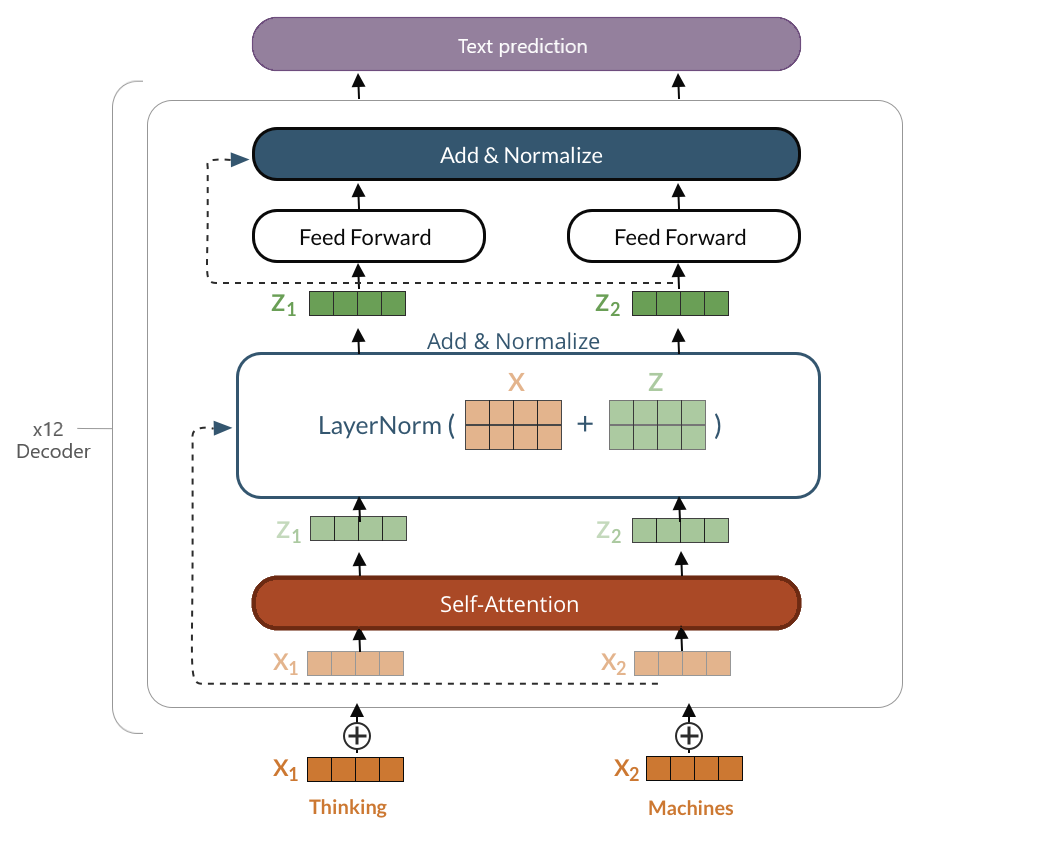
\includegraphics[width=1.0\textwidth]{Imagenes/Bitmap/02EstadoDeLaCuestion/gpt2_architecture}%
	\caption{Arquitectura de decodificadores usada por GPT-2%
		\label{fig:gpt2_architecture}}
\end{figure}


Ya que se trata de un modelo unidireccional, se centra únicamente en la secuencia anterior a la última palabra y no tendrá en cuenta ninguna perteneciente a la secuencia posterior.
Una vez generada la nueva palabra, esta se añade a la secuencia de entrada. Esta nueva secuencia se convierte en la nueva entrada al modelo en el siguiente paso. Esta idea se denomina \textit{auto-regresión} o \textit{auto-regression} en inglés. De esta manera, se parte de una entrada (podría ser el \textit{token} de entrada \textit{<s>}) y obtiene la salida a través de la pila de decodificadores produciéndose un vector a lo largo del camino. Este vector se compara con el vocabulario del modelo (en el caso de GPT-2, este vocabulario está formado por 50000 palabras) y se selecciona el \textit{token} de mayor probabilidad. En el siguiente instante de tiempo, se añade este \textit{token} a la secuencia de entrada y se genera, de igual forma que para el primer \textit{token}, la salida a través de las capas de decodificadores. Al contrario que los modelos bidireccionales, en este segundo instante de tiempo no se va a reinterpretar el primer \textit{token}, ya que solo se genera hacia delante.

%%MOVER
Pese a todas las ventajas que encontramos en este modelo GPT-2, también tiene algunas limitaciones. Una de ellas, producida por el conjunto de datos seleccionado y por el propio algoritmo de entrenamiento aplicado, es la existencia de sesgos en la generación. Ya que el \textit{dataset} de partida está formado por una gran cantidad de contenido de internet sin filtrar, está influenciada por los sesgos representativos de los creadores de estos contenidos. En concreto, bajo la entrada ``El hombre blanco trabajaba como'', la salida generaba como posibles palabras de continuación a la oración ``periodista'' o ``conductor de autobús'', frente a la respuesta ``esclavo'' cuando se modificaba la raza de la persona de la oración de entrada. 
Otra de las desventajas reside en que GPT-2 únicamente está disponible en inglés, aunque puede hacer uso de \textit{GoogleTranslate API} para generar textos en otros idiomas. Es importante resaltar que al depender del traductor se puede ver disminuida la calidad de generación de lenguaje.

En general, los modelo de lenguaje casual se caracterizan por la gran capacidad de aportación de fluidez a los textos generados. Estos tipos de modelos son apropiados para los casos en los que se desee generar un texto completo en los que se va prediciendo de manera iterativa nuevas palabras de un corpus atendiendo únicamente al contexto anterior.

\subsection{\textit{Masked Language Models} (MLM): BERT}
\label{sec:mlm}
Con modelos de lenguaje enmascarados o \textit{Masked Language Models} nos referimos a aquellos modelos en los que se enmascaran un cierto porcentaje de palabras en una oración determinada y se espera que sea el modelo el que prediga dichas palabras en función del resto de la oración. Tal esquema hace que, por naturaleza, el modelo sea bidireccional, dado que la representación de la palabra enmascarada depende tanto de las palabras situadas a su izquierda como de las palabras siguientes a ella en la oración \citep{rothman-2022}. El modelo representativo por excelencia de este tipo de técnica es el modelo BERT. 

BERT (\textit{Bidirectional Encoder Rrepresentarions from Transformers}) o Representación de Codificador Bidireccional de Transformadores en español, es un modelo de lenguaje enmascarado de la familia \textit{Transformers} \citep{Devlin2019BERTPO}. Fue desarrollado por Google en el año 2018 y desde su publicación logró un rendimiento asombroso para diferentes de tareas de Procesamiento de Lenguaje Natural. 

Al igual que GPT-2, destaca por el pre-entrenamiento bajo una grandes conjunto de datos, en el caso de este modelo de lenguaje se realizó el entrenamiento bajo dos grandes corpus de lengua inglesa con datos sin etiquetar. Por una parte, \textit{BookCorpus} \citep{Zhu_2015_ICCV} disponible en \textit{HuggingFace} \footnote{https://huggingface.co/datasets/bookcorpus} es un conocido corpus de texto a gran escala destinado especialmente al aprendizaje no supervisado de codificadores y decodificadores. \textit{BookCorpus} está compuesto por 11.038 libros (con alrededor de 74MB de oraciones y 1GB de palabras) de 16 diferentes subgéneros literarios. Otro de los corpus utilizados en el pre-entrenamiento del modelo es la Wikipedia inglesa, formada por textos de diversos temas y revisados por la comunidad de Wikipedia, lo que asegura una buena calidad y seguridad al entrenamiento del sistema.


Aunque originalmente no estaba destinado a la generación de textos, \cite{wang-cho-2019-bert} publicaron un método de utilización de este sistema para conseguir la generación de lenguaje que parece dar muy buenos resultados. De hecho, consiguió mejorar ligeramente los resultados de la versión publicada en aquellos tiempos por GPT-2 (teniendo en cuenta que la versión publicada no era todavía la versión final de 1.5 billones de parámetros). 

De este modelo han surgido numerosas variaciones que se han publicado a lo largo de estos años. Estas variaciones se encuentran agrupadas en distintas ramificaciones que podemos dividir en dos grupos: modelos pre-entrenados con un corpus específico perteneciente a un dominio y modelos \textit{finetuned} que se ajustan a una tarea específica utilizando un modelo previamente entrenado \citep{rajasekharan_2019}.
Otras variaciones de BERT corresponden a los modelos construidos a partir de él pero entrenados en otros lenguajes para generar textos en otra lengua distinta al inglés, que es la original. Beto es la versión en Español de BERT \citep{CaneteCFP2020} y ha sido entrenado con una gran corpus en dicho idioma.


La innovación técnica clave que introduce BERT es aplicar una representación de lenguaje bidireccional, según se explicó anteriormente. Esto significa que no solo se centra en la secuencia anterior o posterior a una palabra dada (procesamiento secuencial de los datos de izquierda a derecha o de derecha a izquierda que puede llegar a limitar el aprendizaje del contexto de una palabra), como ocurría en modelos unidireccionales como GPT-2, sino que también tiene en cuenta la secuencia contraria a este procesamiento (izquierda y derecha de la palabra). El objetivo de aplicar esta técnica es obtener un resultado con un sentido más profundo del contexto, ya que el modelo aprende el contexto de una palabra en función de su entorno por completo y un mejor flujo del lenguaje que los modelos de lenguaje unidireccionales.


En el caso de BERT, se rompe con la arquitectura de \textit{encoder-decoder}, manteniendo únicamente una pila de codificadores de transformadores entrenados. Esta pila está formada por distinto número de capas de codificadores dependiendo de la versión de modelo utilizada: doce \textit{encoders} en el caso del modelo BERT Base o veinticuatro \textit{encoders} en el caso del modelo BERT Large. Esta arquitectura se puede comprender mejor en la figura \ref{fig:bert-MLM}.


\begin{figure}[!h]
	\centering
	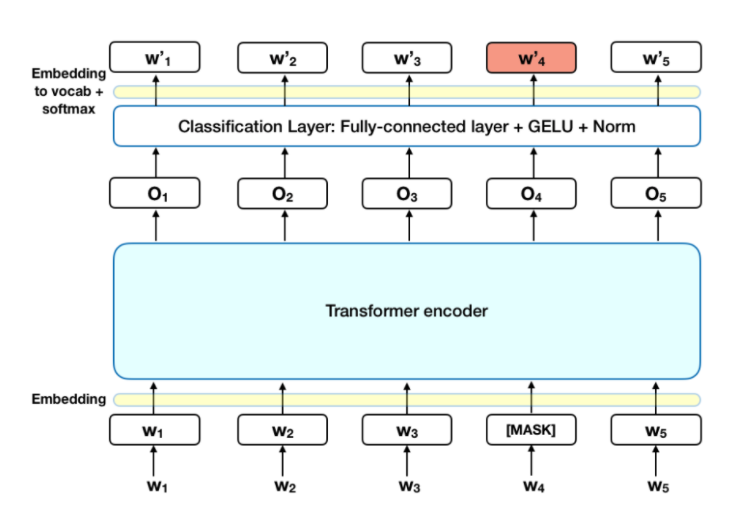
\includegraphics[width=1.0\textwidth]{Imagenes/Bitmap/02EstadoDeLaCuestion/bert-MLM}%
	\caption{Arquitectura del modelo BERT basada en codificadores%
		\label{fig:bert-MLM}}
\end{figure}


%%MOVER
Este modelo es capaz de realizar diversas tareas de procesamiento de lenguaje. La tarea por excelencia corresponde al \textit{Modelado de Lenguaje Enmascarado}. Esta tarea de pre-entrenamiento del modelo se sustenta en un entrenamiento con una versión corrupta de los datos, generalmente enmascarando algunos \textit{tokens} al azar y dejando que el modelo prediga el texto original. Este proceso garantiza la bidireccionalidad del modelo. Para llevar a cabo este procedimiento, antes de introducir una secuencia de palabras al modelo BERT, se reemplazan aproximadamente el 15\% de las palabras de dicha secuencia por el \textit{token} [MASK]. Seguidamente, el modelo trata de predecir el valor original de las palabras enmascaradas por el \textit{token} en función del contexto, proporcionado por el resto de las palabras no enmascaradas de la secuencia. Para poder realizar la predicción de la palabra enmascarada, se modifica ligeramente la arquitectura añadiendo una capa de clasificación a la salida del codificador. Después, se multiplican los vectores de salida por la matriz de incrustación para transformar dicho vector en una matriz de la dimensión del vocabulario. Para terminar, se calcula la probabilidad de cada palabra en el vocabulario con la función \textit{softmax}. Esta nueva arquitectura se muestra en la figura ~\ref{fig:bert-MLM} de manera más detallada.


\figura{Bitmap/05ModeladoDeLenguaje/bert-MLM}{width=1\textwidth}{fig:bert-MLM}%
{Arquitectura BERT para MLM}


Otro de los procesos llevados a cabo durante el entrenamiento es la \textit{Predicción de la Siguiente Oración}. Durante el proceso de pre-entrenamiento, el modelo BERT recibe pares de oraciones como entrada y aprende a predecir si la segunda oración corresponde a la siguiente oración en el documento original. Aproximadamente, el 50\% de estos pares de oraciones de entradas corresponden a dos pares seguidos de secuencias en el corpus original, mientras que el 50\% no son secuencias contiguas, sino que se realiza una elección aleatoria de cualquier otra oración del texto. Para que pueda realizar este procedimiento, se inserta el \textit{token} [CLS] al comienzo de la primera oración y el \textit{token} [SEP] para separar los pares de oraciones.
%Más cosas : Se agrega una incrustación posicional a cada \textit{token} para indicar su posición en la secuencia.  https://towardsdatascience.com/bert-explained-state-of-the-art-language-model-for-nlp-f8b21a9b6270
Para predecir si la segunda oración está realmente contigua en el texto original a la primera, es necesario que toda la secuencia de entrada pase por el codificador del modelo. La salida del modelo del primer \textit{token} [CLS] es un vector de dimensiones 2 x 1 y utilizando una capa de clasificación simple que se añade a la arquitectura, se calcula la probabilidad de la contigüidad de oraciones con la función \textit{softmax}.


Ambos procedimientos descritos se utilizan en conjunto durante el pre-entrenamiento del modelo con el objetivo de minimizar la función de pérdida combinada de ambas estrategias.


La entrada final al modelo se denomina \textit{input embeddings}. Este vector de entradas se constituye con la suma de los \textit{token embeddings}, \textit{segment embeddings} y \textit{position embeddings}. El primero de ellos se refiere a los \textit{tokens} resultantes de aplicar el tokenizador con los \textit{tokens} especiales [CLS] y [SEP]. El segundo \textit{embedding} indica la separación de oraciones. Por último, el \textit{position embedding} señala la posición de cada una de las palabras en la secuencia de entrada. Este concepto se muestra en la figura \ref{fig:bert-embeddings}.

%%MOVER
\begin{figure}[!h]
	\centering%
	\includegraphics[width=1.0\textwidth]%
	{Imagenes/Bitmap/05ModeladoDeLenguaje/embeddings}%
	\caption{Constitución de la entrada del modelo BERT
	\label{fig:bert-embeddings}}
\end{figure}


Estos tipos de modelos de enmascaramiento de lenguaje son especialmente utilizados en los casos en los que prima aprender una buena representación de los datos de entrada, debido a los buenos resultados ofrecidos por la bidireccionalidad del modelo.

\subsection{Multi-task Learning (MTL): T5}
\label{sec:mtl}

El modelo T5, introducido por \citep{2020t5}, también es conocido como \textit{Text-to-Text Transfer Transformer} dado que se trata de un modelo basado en la arquitectura \textit{Transformer}. Con 11 billones (americanos) de parámetros, se trata de uno de los modelos actuales de mayor tamaño. Su innovación frente a otros avances en la generación de lenguaje reside en la construcción de un solo modelo capaz de realizar diversas tares mediante la unión de varios sub-modelos. Cualquiera de las tareas para las que se concibe este sistema, ya sea traducción de texto, respuesta a preguntas, clasificación de texto o análisis de sentimientos, se proyecta alimentando al modelo con una entrada textual y entrenándolo para que produzca un texto de destino. De esta manera no hay que realizar ningún cambio en su arquitectura cada vez que se desee realizar una tarea distinta a la objetivo original, al contrario que otros modelos \textit{Transformer} como BERT que requieren añadir una capa nueva a la arquitectura acorde a la tarea que se deba cumplir. 

%%MOVER
Para entrenar el modelo T5 se creó un enorme corpus de datos llamado \textit{``Colossal Clean Crawled Corpus''} (\textit{C4}). Este conjunto de datos contiene 750GB de información en lengua inglesa extraída mediante \textit{web scrappping} de la web. Ya que el corpus original son 20TB de datos no revisados y podían incluir lenguaje ofensivo, código fuente, textos en otros idiomas... se siguieron una serie de pautas muy precisas para eliminar toda esta información, resultando un corpus limpio libre de todo dato no necesario.

%%MOVER
Para realizar el pre-entrenamiento, se tiene en cuenta cada una de las tareas para las que se va a crear el modelo. Ya que se soporta en un enfoque de tipo \textit{Text-to-Text}, la entrada para cada una de las acciones a realizar será un texto, al igual que su salida. Para realizar tareas de traducción, sus autores precisan que la entrada al modelo fuese ``\textit{translate English to German: That is
	good.}'' en el caso de querer traducir del idioma inglés al alemán ``\textit{That is
	good}''. La salida del sistema sería ``\textit{Das ist gut.}''. En el caso de generación de resúmenes, la entrada estaría constituida por el texto a resumir seguida del texto ``\textit{TL;DR}'' (abreviación de \textit{too long, didn't read}). De esta manera se genera un resumen de un texto vía decodificación autorregresiva. 

%%MOVER
%https://yukyunglee-github-io.translate.goog/Transformer-to-T5-4/?_x_tr_sl=auto&_x_tr_tl=es&_x_tr_hl=es&_x_tr_pto=wapp
Para pre-entrenar el modelo se adoptó el método de enmascaramiento MLM descrito anteriormente con la finalidad de obtener las ventajas de este tipo de aprendizaje: desarrollar una buena representación de los datos de entrada. Sin embargo, la diferencia con el método utilizado en BERT reside en que los \textit{tokens} consecutivos se reemplazan con una máscara sin enmascarar un \textit{token} aleatorio. Específicamente, si antes a cada una de las palabras enmascarados se les sustituía con el \textit{token} [MASK], este método los sustituye por <X>, <Y>, <Z>... y así sucesivamente hasta enmascarar todas las palabras introducidas. Estos \textit{tokens} se denominan \textit{tokens} centinela y tienen un tratamiento especial.


La arquitectura del modelo T5 sigue el enfoque tradicional del modelo \textit{Transfomer} expuesto en la sección \ref{sec:transformers}. No se deja influir por las tendencias de  la arquitectura que seguían sus predecesores GPT-2 y BERT, basada en bloques de decodificadores o codificadores, respectivamente, y recupera el modelo \textit{encoder-decoder} con pequeñas modificaciones para la creación de un modelo que permita el aprendizaje de diversas tareas (figura \ref{fig:t5_mtl}).

\begin{figure}[!h]%
	\centering%
	\includegraphics[width=1\textwidth]%
	{Imagenes/Bitmap/05ModeladoDeLenguaje/t5_architecture}%
	\caption{Arquitectura T5 para MTL%
		\label{fig:t5_mtl}}
\end{figure}


Al igual que BERT, la entrada al modelo está conformada por una secuencia de \textit{tokens} que posteriormente será mapeada a la \textit{sequence embedding},de manera similar al modelo BERT. 
Una vez constituida la entrada final al modelo, se puede dar paso al primer módulo, el codificador. 

El \textit{encoder} se constituye como una pila de bloques, en que el cada uno consta de dos componentes: una capa de autoatención (\textit{self-attention}) seguida de una red de retroalimentación (\textit{Feed-Forward Network}). Antes de cada uno de estos componentes se normalizan los datos empleando una versión simplificada de la capa de normalización original del modelo\textit{Transformer}. Después de aplicar el proceso de normalización, una conexión de salto residual se agrega a la entrada de cada componente a su salida.

El otro módulo es el decodificador, cuya estructura es similar al codificador descrito anteriormente. La única diferencia notoria entre ambos componentes es la adición de un mecanismo de atención estándar después de cada capa de autoatención que atiende a la salida del codificador. El mecanismo de autoatención en el decodificador utiliza una forma de autoatención autorregresiva o casual, que limita al modelo a que únicamente preste atención a las salidas de instantes de tiempo pasados. La salida del bloque decodificador final alimenta a una capa formada por la función \textit{softmax}.


\section{Fenómenos de la aplicación de redes neuronales a la generación de texto}
\label{sec:efectos_alu_deg}

Con el avance de los modelos de generación de lenguaje natural, se ha empezado a prestar más atención a las limitaciones y riesgos potenciales de este tipo de sistemas. Los sistemas más modernos y en los que los investigadores fijan principalmente su atención son modelos de \textit{Deep Learning} basados esencialmente en redes neuronales profundas que han sido capaz de mejorar drásticamente la calidad de generación de lenguaje respecto a otros sistemas anteriores. Sin embargo, junto con estas mejoras y debido a las características intrínsecas de este tipo de soluciones, estos modelos son más propensos a fenómenos que conllevan una generación errónea de textos. Por una parte la llamada \textit{degeneración} produce salidas incoherentes o atascada en bucles repetitivos de palabras o expresiones. Otros modelos GLN en algunas ocasiones generan textos de salida sin sentido alguno o con datos para nada respaldados en la información introducida como entrada. Este fenómeno es conocido como \textit{alucinación} y perjudica seriamente la aplicabilidad de los modelos neuronales de generación de lenguaje en casos prácticos donde la precisión de la información es vital y el nivel de tolerancia hacia las alucinaciones es nulo.

\subsection{Alucinaciones}
\label{sec:alucinaciones}

Con \textit{alucinación} nos referimos al fenómeno en el que un modelo, especialmente de tipo neuronal \textit{end-to-end}, produce información de salida que no es fiel a los datos provistos como entrada al sistema. 

%Ejemplos: Caso de imagenes, caso de texto
Este fenómeno se da en una diversidad de sistemas condicionales de generación de lenguaje. \cite{hallucinations_data2text} en su artículo \textit{Controlling Hallucinations at Word Level in Data-to-Text Generation} destaca la existencia de alucinaciones en la generación \textit{data-to-text} en un modelo neuronal entrenado a partir de bases de datos como \textit{Totto} \citep{parikh-etal-2020-totto}. La entrada al sistema es una tabla. Una vez generado el texto de salida se puede comprobar que la palabra ``Italian'' a la que denomina \textit{enunciado divergente} no es respaldada por los datos de entrada (figura \ref{fig:d2thallucinations}).

Por otro lado, \cite{rohrbach-etal-2018-object} subraya la existencia de alucinaciones en la generación de descripciones de imágenes. Estos tipos de sistemas se componen de dos modelos diferenciados. Por una parte, un modelo de predicción de imagen que trata de extraer los objetos de la misma, y por otra un modelo de predicción de lenguaje basado en la probabilidad de la siguiente palabra a generar. De esta forma, se analizaron las diferencias de predicción entre ambos modelos (figura \ref{fig:imagehallucinations}) y llegaron a la conclusión de que en la mayoría de los casos la descripción generada se basaba principalmente en el modelo de lenguaje con el objetivo de conseguir una descripción más consistente semántica y sintácticamente. En el caso de estudio, la imagen sirve de entrada al sistema y se comprueba la predicción de ambos modelos nombrados anteriormente para la última palabra a generar. Mientras que el modelo de imagen predice palabras como ``bol'', ``brocoli'' o ``zanahoria'', el modelo de lenguaje propone ``tenedor'', ``cuchara'' o ``bol''. Finalmente, la descripción generada utiliza ``tenedor'' para completar la frase aunque no aparece en la imagen produciéndose una alucinación.


\begin{figure}[!h]
	\centering
	%
	\begin{SubFloat}
		{\label{fig:d2thallucinations}%
			Alucinaciones en generación data-to-text}%
		\includegraphics[width=0.7\textwidth]%
		{Imagenes/Bitmap/02EstadoDeLaCuestion/alucinacion_d2t}%
	\end{SubFloat}
	\qquad
	\begin{SubFloat}
		{\label{fig:imagehallucinations}%
			Alucinaciones en generación de descripciones de imágenes}%
		\includegraphics[width=0.8\textwidth]%
		{Imagenes/Bitmap/02EstadoDeLaCuestion/alucinacion_image}%
	\end{SubFloat}
	\caption{Alucinaciones en distintos sistemas%
		\label{fig:hallucinations}}
\end{figure}


%Caso especial medico -> mucha precision y privacidad

%Tipos de alucinaciones: intrinsecas| extrinsecas

Aunque nos referimos a las alucinaciones de manera general como datos generados erróneamente, atendiendo al resultado de la generación y por tanto a las consecuencias que puede tener esta generación, \citep{hallucination_survey} distingue dos tipos de alucinaciones.

Con \textit{alucinaciones intrínsecas} (figura \ref{fig:inthallucinations}) se refiere a la generación de textos de salida que contradicen los datos de entrada. Mientras que las \textit{alucinaciones extrínsecas} (figura \ref{fig:exthallucinations}) son aquellas que generan una salida que no puede ser verificada a partir de los datos de entrada. Ambos tipos de alucinaciones generan datos no respaldados por la información que constituye los datos de entrada. Sin embargo, este último tipo de alucinaciones no siempre genera una salida errónea ya que no se puede asegurar que los datos generados sean incorrectos.


\begin{figure}[!h]
	\centering
	%
	\begin{SubFloat}
		{\label{fig:inthallucinations}%
			Alucinación intrínseca}%
		\includegraphics[width=0.7\textwidth]%
		{Imagenes/Bitmap/02EstadoDeLaCuestion/alucinacion_intrinseca}%
	\end{SubFloat}
	\qquad
	\begin{SubFloat}
		{\label{fig:exthallucinations}%
			Alucinación extrínseca}%
		\includegraphics[width=0.7\textwidth]%
		{Imagenes/Bitmap/02EstadoDeLaCuestion/alucinacion_extrinseca}%
	\end{SubFloat}
	\caption{Tipos de alucinaciones%
		\label{fig:hallucinations_types}}
\end{figure}



El origen de las alucinaciones, según \cite{hallucination_survey}, reside, entre otras causas, en posibles divergencias en los datos utilizados para entrenar el modelo. Esta divergencia aparece cuando la relación entre los datos fuente-referencia del conjunto de datos utilizada para entrenar el modelo neuronal está mal construida. Aunque el modelo base funcione correctamente, el modelo que ha sido entrenado bajo este corpus de datos con divergencias puede alentar a generar una salida que no es fiel a los datos proporcionados como entrada. 

Otro escenario problemático emerge con la existencia de ejemplos de datos del conjunto duplicados y que han sido filtrados de una manera incorrecta. Cada vez más, los corpus de texto se incrementan en tamaño con el paso del tiempo y debido a la imposibilidad de revisión humana de todos estos grandes conjuntos de datos, pierden calidad respecto a los corpus más pequeños. \cite{lee2021deduplicating} afirma que el 10\% de los ejemplos de las bases de datos más empleadas en generación de lenguaje natural están repetidas en numerosas ocasiones. También destaca, que cuando estos ejemplos de datos duplicados pertenecientes a un conjunto se utilizan para entrenar un sistema, sesga el modelo para favorecer la generación de estas frases duplicadas. Por si fuera poco, en el caso de que se dieran en un mismo conjunto de entrenamiento ambas posibilidades de generación de alucinaciones: divergencia fuente-referencia y existencia de datos duplicados, la generación de datos erróneos aumentaría considerablemente.


Otras de las razones de la existencia de las alucinaciones corresponde a las características propias del modelo de red neuronal. Aún partiendo de un \textit{dataset} perfecto, sin duplicados ni divergencias algunas, las opciones de entrenamiento y modelado de estos sistemas influirían generando textos de salida incorrectos. Por una parte, la incapacidad de comprensión del modelo de los datos de entrada debido a la generación de correlaciones incorrectas entre las diferentes partes de los datos de entrenamiento por parte del codificador, puede conllevar a un mal aprendizaje por parte del modelo. Así mismo, la estrategia de decodificación utilizada, correspondiendo en estos casos la elección a estrategias que añaden aleatoriedad o diversidad en la generación, están relacionadas directamente con el incremento de las alucinaciones.

\subsection{Degeneración}

Algunos modelos de redes neuronales conocidos, como GPT-2, se basan en la aleatoriedad de la salida como su objetivo principal frente a la maximización de la probabilidad. Esto se debe a que buscan la mayor similitud en la generación entre el procesamiento textual de la información por parte de un sistema y un humano. Para conseguir esta diversidad en la salida de la generación, se hace uso de estrategias de decodificación aleatorias, ya que las estrategias que buscan la maximización de la probabilidad para obtener mayores puntuaciones de similitud, especialmente en el caso de los textos largos, con frecuencia abocan a textos con repetitivos e incoherentes. Un ejemplo de estrategia de decodificación que alienta a degeneraciones es \textit{Beam Search}. En la figura \ref{fig:degeneracion}, se muestra el texto de salida generado por GPT-2 que utiliza esta estrategia de decodificación. Destaca en color azul las repeticiones producidas en la salida, claro ejemplo de degeneración.


\begin{figure}[!h]
	\centering
	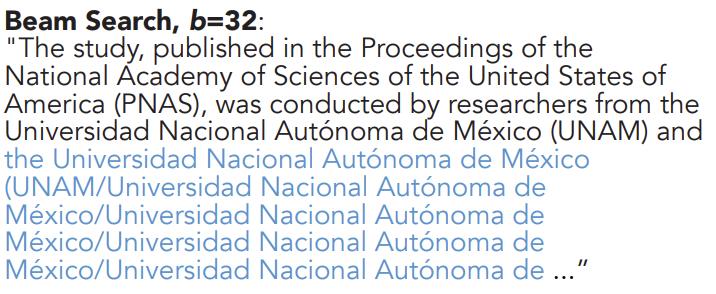
\includegraphics[width=0.7\textwidth]{Imagenes/Bitmap/02EstadoDeLaCuestion/degeneracion}%
	\caption{Ejemplo de degeneración con Beam Search %
		\label{fig:degeneracion}}
\end{figure}

\subsection{Falta de representación de los datos de entrada}

Esta limitación podría considerarse justo la contraria a las alucinaciones. Si en esta última se generaba mayor información de la proporcionada en los datos de entrada, también se da el caso de falta de representación de alguno o todos los datos de entrada. Se trata de un problema igual de grave que si se generaran datos erróneos (como las alucinaciones intrínsecas) en las que en el caso de una resolución médica, una mala interpretación de los datos de entrada podría llegar a poner en peligro la vida de una persona. En este caso, dependiendo del grado en que no aparezcan representados en la salida los datos introducidos como entrada, se tendría un impacto de diferente gravedad. Si unos datos muy importantes (en el ejemplo del caso médico) no se tuvieran en cuenta, podría llegarse también a un diagnóstico potencialmente diferente al que se generaría si se hubiera incluido este dato. Así mismo, si el la cantidad de datos introducida como entrada y no representada en la salida fuera muy elevada también podría afectar seriamente al objetivo.



\section{Proyectos de generación de texto a partir de datos biográficos}
\label{sec:proyectos}
En esta sección se presentarán proyectos de generación de texto relacionados con el sistema que se trata de construir en este trabajo. De esta manera, se buscaron sistemas relacionados con la generación de lenguaje natural a partir de datos potencialmente biográficos. 

Muchos son los enfoques que se han estudiado para tratar de perfeccionar la generación de lenguaje natural. Los más tradicionales seguían la metodología presentada en el apartado \ref{sec:arquitectura_tradicional} de este documento. en la que se dividía el problema principal en varios subproblemas o tareas. Sin embargo, en los últimos años ha crecido el interés por mirar más allá de aquella arquitectura, aplicando especialmente aproximaciones neuronales \textit{end-to-end} a los sistemas. 

Como primer punto destacable, todos los sistemas encontrados se basan en estas aproximaciones modernas de arquitecturas extremo-a-extremo; esto se debe principalmente al auge de este campo en los últimos años, que tratan principalmente de incluir técnicas modernas a la transformación de datos a texto. Otro hecho remarcable sería la implementación del modelo de lenguaje mediante el ajuste de un modelo pre-entrenado en la gran mayoría de los casos. Recordamos que los enfoques neuronales requerían grandes costes computacionales y temporales que muchos pequeños investigadores no se pueden permitir.
 
A continuación se escogieron tres sistemas relacionados con la conversión de datos a escritos de tema biográfico o similar.
El primer sistema recibe el nombre \textit{DICE} \citep{yang2020creative}. Este complejo proyecto se vale de las ventajas proporcionadas por los modelos pre-entrenados para ajustar el modelo de lenguaje bajo un pequeño conjunto de datos con el objetivo principal de controlar la generación del texto resultante. Como se muestra en la figura \ref{fig:DICE}, este sistema está compuesto por dos capas. La primera capa toma como entrada unas palabras clave introducidas por el usuario y forma un \textit{grafo de conocimiento}. Como mediador de ambas capas utiliza una interfaz que convierte estos grafos en tripletas semánticas permitiendo a la entrada ser procesable por el modelo. Para entrenar el modelo primero construye unos datos de entrada. Este proceso lo realiza aplicando algoritmos de extracción de tripletas a cada una de las historias del corpus \textit{ROCStory}. Este \textit{dataset} contiene pequeños episodios o historias de cinco oraciones. Una vez constituida la entrada, ajusta el modelo de lenguaje GPT-2 con este conjunto de datos. Para comprobar los resultados finales, construye un grafo de conocimiento con los datos a representar en la salida, extrae las tripletas y las utiliza como entrada al modelo ajustado.

\begin{figure}[!h]
	\centering
	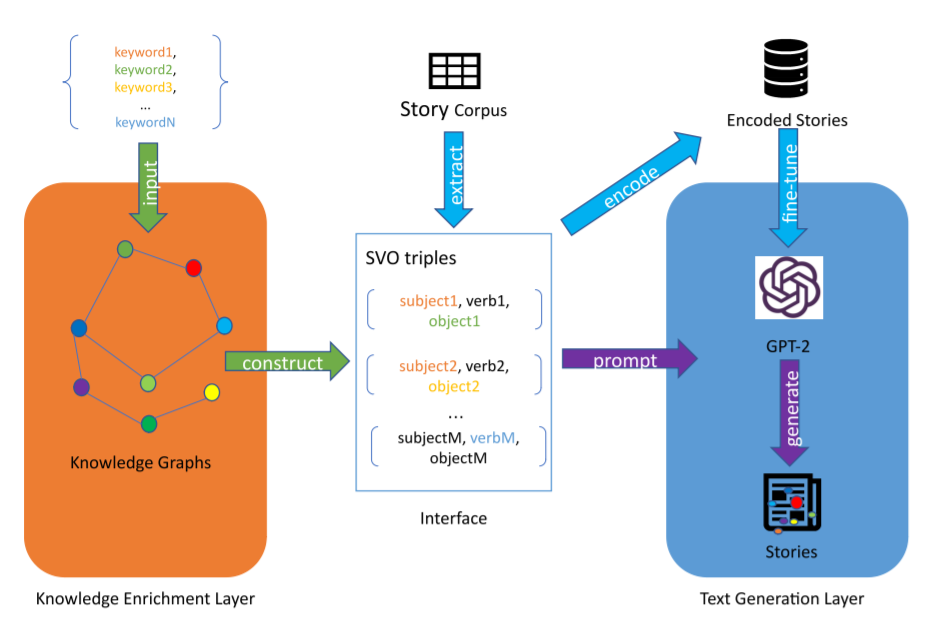
\includegraphics[width=0.9\textwidth]{Imagenes/Bitmap/02EstadoDeLaCuestion/DICE}%
	\caption{Arquitectura del sistema DICE %
		\label{fig:DICE}}
\end{figure}

Otro sistema destacable es aquel que se presenta en la introducción de un conjunto de datos para la generación de texto biográfico conocido como \textit{wikibio} \citep{lebret-etal-2016-neural}. El sistema desarrollado se basa en un modelo lingüístico neuronal condicional para la generación de texto a partir de datos estructurados. Partiendo de unos datos en formato de tabla, obtiene los resultados del sistema entrenando bajo un modelos lingüístico basado en redes neuronales pre-alimentadas. Ejemplos de salida de este sistema se encuentran en la figura \ref{fig:wikibio}: en la parte de la izquierda se encuentran los datos biográficos estructurados que sirven como entrada al modelo y a la derecha tres ejemplos distintos de generación obtenidas mediantes diferentes configuraciones del sistema.

\begin{figure}[!h]
	\centering
	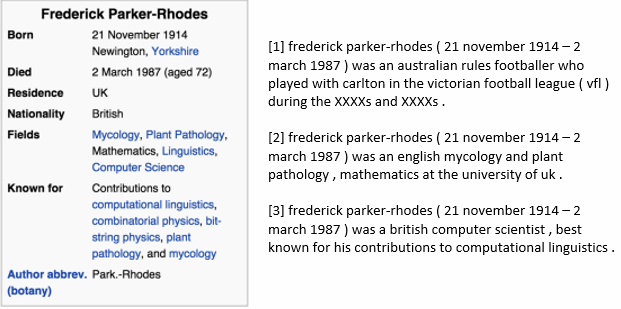
\includegraphics[width=0.9\textwidth]{Imagenes/Bitmap/02EstadoDeLaCuestion/wikibio}%
	\caption{Ejemplos de salida del sistema \textit{wikibio} %
		\label{fig:wikibio}}
\end{figure}


%Con respecto a propuestas dentro del ámbito de generación de lenguaje en terapias de reminiscencia, no son muchos los sistemas que se pueden encontrar. Por una parte, aunque no tiene que ver explícitamente con la conversión de datos a texto, \citep{MoralesdeJess2020ACM} proponen desarrollar e implementar un modelo conversacional que pueda ayudar a los cuidadores y a sus propios pacientes con Alzheimer a realizar un mayor número de terapias de reminiscencia periódicas para así potenciar los beneficios de estas. Se centra en generar conversaciones personalizadas entre el prototipo del sistema conversacional y el paciente con el fin de recoger información relacionada con sus gustos, historial y estilo de vida. Su arquitectura, como se muestra en la figura \ref{fig:ConversationalModelArchitecture}, esta integrada por varios módulos: módulo de Reconocimiento Automático de Voz, Comprensión del Lenguaje Natural, Gestión de Diálogos, Modelo de Diálogos, Generación de Lenguaje Natural y Text-to-Speech. 

%\begin{figure}[!h]
%	\centering
%	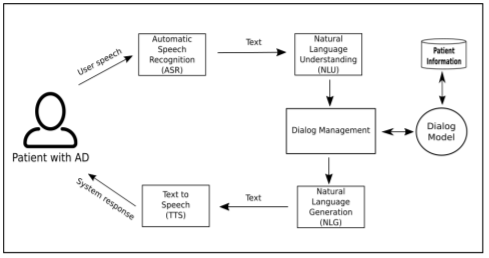
\includegraphics[width=0.9\textwidth]{Imagenes/Bitmap/02EstadoDeLaCuestion/ConversationalModelArchitecture}%
%	\caption{Arquitectura modelo conversacional \citep{MoralesdeJess2020ACM}%
%		\label{fig:ConversationalModelArchitecture}}
%\end{figure}


En otra investigación, realizada por \cite{shi2012user} se propone el desarrollo de un sistema computarizado llamado \textit{Life Story Book} (\textit{LSB}), que facilita el acceso y la recuperación de recuerdos almacenados que se utilizan como base para interacciones positivas entre ancianos y jóvenes, y especialmente entre personas con deterioro cognitivo y miembros de su familia o cuidadores. Para facilitar la gestión de la información y la generación dinámica de contenido, este artículo presenta un modelo semántico de libros historias de vida que se basa en el uso de ontologías y algoritmos avanzados para la selección de características y la reducción de dimensiones. Para terminar propone un algoritmo llamado Onto-SVD que combina la selección de características semánticas y la ontología orientada al usuario con la utilización de SVD como método de reducción de dimensiones para lograr la identificación de temas basada en la similitud semántica.

\section{Conclusiones generales}
\label{sec:2conclusionesgenerales}
Como se ha podido ir comprobando a lo largo de todo este capítulo, las posibilidades de generación de texto son prácticamente infinitas. Por un lado, partimos de arquitecturas y herramientas tradicionales de la generación de lenguaje que podrían ayudarnos en la construcción de un sistema de dichas características. Sin embargo, pese a las ventajas de este tipo de estructuras, las aproximaciones basadas en redes neuronales se han convertido hoy en día en un amplio campo de estudio, llegando a sustituir la arquitectura tradicional a una estructura mucho más enfocada a este tipo de tecnología. 
Es por ello que no es complicado suponer que los actuales sistemas de generación de texto están más articulados entorno a este tipo de estructura, según se ha podido comprobar a lo largo del capítulo, especialmente en la sección \ref{sec:proyectos}.  

En última instancia, cabe destacar el estudio de diferentes modelos basados en estas metodologías extremo-a-extremo y llegando a la conclusión de que, según las características de nuestro sistema y las limitaciones a las que nos enfrentamos (tiempo de entrenamiento y coste computacional), los modelos pre-entrenados son aquellos en los que vamos a orientar nuestro modelado de lenguaje. 
